% =====================================================================
%  Reporte de laboratorio - Proyecto Final de Arquitecturas Computacionales
%  Semaforo inteligente con un procesador RISC-V en la FPGA DE10-Lite
%  Compilar con pdfLaTeX (Overleaf: Menu -> Compiler -> pdfLaTeX)
% =====================================================================
\documentclass[12pt,letterpaper]{article}

% ---------------------------------------------------------------------
% Si Overleaf dice que el proyecto necesita mas tiempo de compilacion,
% cambia \codigotrue por \codigofalse: el reporte compila sin los
% apendices de codigo, y el codigo se entrega aparte compilando
% anexo_codigo.tex (Menu -> Main document -> anexo_codigo.tex).
% ---------------------------------------------------------------------
\newif\ifcodigo
\codigotrue

% Paquetes y estilo compartidos por main.tex y anexo_codigo.tex
\usepackage[utf8]{inputenc}
\usepackage[T1]{fontenc}
\usepackage[spanish,es-tabla,es-noshorthands,es-nodecimaldot]{babel}
\usepackage{lmodern}
\usepackage[margin=2.5cm]{geometry}
\usepackage{graphicx}
\usepackage{float}
\usepackage{booktabs}
\usepackage{array}
\usepackage{longtable}
\usepackage{multirow}
\usepackage[table]{xcolor}
\usepackage{listings}
\usepackage{caption}
\usepackage{amsmath}
\usepackage{enumitem}
\usepackage{fancyhdr}
\usepackage[hidelinks]{hyperref}

% ---------- Datos del equipo (llenar) ----------
\newcommand{\universidad}{Universidad de las Américas Puebla}
\newcommand{\facultad}{Departamento de Computación, Electrónica y Mecatrónica}
\newcommand{\materia}{Arquitecturas Computacionales}
\newcommand{\profesor}{Omar Guillén Fernández}
\newcommand{\fechaentrega}{1 de diciembre de 2026}

% ---------- Estilo ----------
\DeclareRobustCommand{\cod}[1]{\texttt{\detokenize{#1}}}
\setlength{\parskip}{0.5em}
\captionsetup{font=small,labelfont=bf}
\renewcommand{\arraystretch}{1.2}

\pagestyle{fancy}
\fancyhf{}
\lhead{\small Proyecto Final -- \materia}
\rhead{\small Semáforo inteligente RISC-V}
\cfoot{\thepage}

\definecolor{fondo}{RGB}{248,248,248}
\definecolor{comentario}{RGB}{0,128,0}
\definecolor{clave}{RGB}{0,0,180}
\definecolor{cadena}{RGB}{163,21,21}

\lstset{
  basicstyle=\ttfamily\scriptsize,
  backgroundcolor=\color{fondo},
  keywordstyle=\color{clave}\bfseries,
  commentstyle=\color{comentario}\itshape,
  stringstyle=\color{cadena},
  numbers=left, numberstyle=\tiny\color{gray}, numbersep=6pt,
  frame=single, rulecolor=\color{gray!50},
  breaklines=true, breakatwhitespace=false,
  tabsize=4, showstringspaces=false,
  columns=fullflexible, keepspaces=true,
  captionpos=t
}
\lstdefinelanguage{RISCV}{
  morekeywords={add,sub,and,or,xor,slt,sll,srl,sra,mul,addi,andi,ori,xori,slti,
    slli,srli,srai,lw,sw,beq,bne,blt,jal,jalr,lui,nop},
  sensitive=false,
  morecomment=[l]{\#}
}
\renewcommand{\lstlistingname}{Código}
\renewcommand{\lstlistlistingname}{Índice de códigos}



\begin{document}

% =====================================================================
%  PORTADA
% =====================================================================
\begin{titlepage}
  \centering
  {\Large \textbf{\universidad}\par}
  \vspace{0.3cm}
  {\large \facultad\par}
  \vspace{1.5cm}
  {\large \materia\par}
  \vspace{0.5cm}
  {\Large Proyecto Final\par}
  \vspace{1.2cm}
  \rule{\linewidth}{0.8pt}\par
  \vspace{0.4cm}
  {\huge \textbf{Semáforo inteligente basado en un procesador RISC-V implementado en la FPGA DE10-Lite}\par}
  \vspace{0.4cm}
  \rule{\linewidth}{0.8pt}\par
  \vspace{1.5cm}
  {\large \textbf{Integrantes}\par}
  \vspace{0.3cm}
  \begin{tabular}{ll}
    Juan Diego Acosta Ojeda & 185015 \\
    Mario Cardeña García & 180220 \\
  \end{tabular}
  \vfill
  {\large \textbf{Profesor:} \profesor\par}
  \vspace{0.3cm}
  {\large \textbf{Fecha de entrega:} \fechaentrega\par}
\end{titlepage}

% =====================================================================
%  RESUMEN E ÍNDICES
% =====================================================================
\begin{abstract}
En este proyecto se diseñó, describió en Verilog y verificó por simulación un procesador
RISC-V de 32 bits con microarquitectura multiciclo. Este procesador controla un
\emph{semáforo inteligente} para el cruce de una avenida principal con una calle secundaria,
con paso peatonal. El procesador se construyó reutilizando los módulos desarrollados en clase
(ALU \cod{alu_riscv}, sumador, multiplexor, registro PIPO, ROM, RAM y la unidad de control
\cod{uc_simple}), a los que se agregaron un banco de registros, un generador de inmediatos y una
unidad de control extendida. El semáforo es un programa en ensamblador RISC-V almacenado
en la ROM, que interactúa con la tarjeta Terasic DE10-Lite por medio de periféricos mapeados
en memoria: un sensor de autos (\cod{SW[0]}), un botón peatonal (\cod{KEY[1]}), un modo de
emergencia que pone todos los semáforos en rojo (\cod{SW[1]}) y una cuenta regresiva en los
displays de siete segmentos. Las luces se muestran en los LEDs de la tarjeta y también en LEDs
rojos, amarillos y verdes montados en una protoboard y conectados al puerto GPIO. Se
escribieron cuatro bancos de prueba (\emph{testbenches}) y se simularon en Aldec Active-HDL. El
procesador ejecutó correctamente las 25 instrucciones soportadas (27 de 27 verificaciones) y el sistema completo pasó todos los escenarios de prueba:
operación normal, demanda vehicular, solicitud peatonal y emergencia.
\end{abstract}

\newpage
\tableofcontents
\newpage
\listoffigures
\listoftables
\newpage

% =====================================================================
\section{Introducción}
% =====================================================================
Los semáforos de tiempo fijo reparten el tiempo de verde con un ciclo predeterminado, sin tomar
en cuenta si realmente hay vehículos o peatones esperando. En cruces donde una avenida principal
con mucho tránsito se cruza con una calle secundaria con poco tránsito, esto provoca esperas
innecesarias: la avenida se detiene aunque nadie quiera cruzar. Un \emph{semáforo inteligente}
(o \emph{actuado}) usa sensores y botones para decidir cuándo cambiar de fase. Además debe poder
atender situaciones especiales, como el paso de un vehículo de emergencia.

El objetivo del curso de Arquitecturas Computacionales es entender cómo está construido un
procesador por dentro. Por ello, en lugar de resolver el semáforo únicamente con una máquina de
estados, se decidió construir un \textbf{procesador RISC-V} completo y escribir la lógica del
semáforo como un \textbf{programa}. Así, el mismo hardware podría ejecutar otro comportamiento
con solo cambiar el contenido de la memoria de instrucciones, que es la idea central de la
arquitectura de von Neumann/Harvard de programa almacenado.

El sistema se describió en Verilog, se simuló en Aldec Active-HDL (versión estudiantil) y se
preparó para implementarse en la tarjeta Terasic DE10-Lite, que tiene un FPGA Intel MAX~10.
El reporte está organizado así: la Sección~\ref{sec:objetivos} presenta los objetivos; la
Sección~\ref{sec:marco} el marco teórico; la Sección~\ref{sec:materiales} los materiales; la
Sección~\ref{sec:desarrollo} el diseño del procesador, de los periféricos y del programa; la
Sección~\ref{sec:resultados} los resultados de simulación; la Sección~\ref{sec:analisis} su
análisis, y la Sección~\ref{sec:conclusiones} las conclusiones. En los apéndices se incluye el
código completo, que también está disponible en el repositorio del proyecto~\cite{repo}.

% =====================================================================
\section{Objetivos}\label{sec:objetivos}
% =====================================================================
\subsection{Objetivo general}
Diseñar e implementar en Verilog un procesador RISC-V multiciclo que, ejecutando un programa
almacenado en memoria, controle un semáforo inteligente operable desde la tarjeta FPGA DE10-Lite.

\subsection{Objetivos específicos}
\begin{enumerate}[itemsep=0pt]
  \item Reutilizar e integrar los módulos desarrollados en clase (ALU, sumador, multiplexor,
        registro, ROM, RAM y unidad de control) en la ruta de datos de un procesador.
  \item Implementar un subconjunto de la arquitectura RV32I (más la instrucción \cod{mul}) con
        instrucciones de los seis formatos: R, I, S, B, U y J.
  \item Diseñar periféricos mapeados en memoria para leer interruptores y botones y para
        controlar LEDs y displays de siete segmentos.
  \item Programar en ensamblador RISC-V un semáforo con sensor de autos, botón peatonal, modo de
        emergencia y cuenta regresiva.
  \item Verificar cada módulo y el sistema completo con \emph{testbenches} autoverificables en
        Active-HDL, y documentar las formas de onda obtenidas.
  \item Preparar los archivos de Quartus Prime (asignación de pines y restricciones de tiempo)
        para programar la DE10-Lite.
\end{enumerate}

% =====================================================================
\section{Marco teórico}\label{sec:marco}
% =====================================================================

\subsection{FPGA y la tarjeta DE10-Lite}
Un FPGA (\emph{Field Programmable Gate Array}) es un circuito integrado formado por miles de
bloques lógicos configurables (tablas de búsqueda o LUT y \emph{flip-flops}), bloques de memoria
y multiplicadores, unidos por una red de interconexión programable. Al sintetizar una
descripción de hardware, la herramienta (Quartus Prime, en el caso de Intel) traduce el diseño a
esos recursos y genera un archivo de configuración.

La tarjeta Terasic DE10-Lite tiene un FPGA Intel MAX~10 \cod{10M50DAF484C7G} con cerca de
50\,000 elementos lógicos, bloques de memoria M9K de 9\,kbit, un oscilador de 50~MHz, 10
interruptores deslizables (\cod{SW}), 2 botones (\cod{KEY}, activos en bajo), 10 LEDs rojos
(\cod{LEDR}) y 6 displays de siete segmentos (\cod{HEX0}--\cod{HEX5}) de ánodo común, es decir,
cada segmento se enciende con un \texttt{0} lógico~\cite{de10lite,max10}.

\subsection{Verilog HDL}
Verilog es un lenguaje de descripción de hardware estandarizado en IEEE~1364~\cite{ieee1364}.
Un diseño se divide en \emph{módulos} con puertos de entrada y salida, que pueden instanciarse
dentro de otros módulos (diseño jerárquico), como se hizo en clase con el
\cod{full_adder_instantiated}. La lógica combinacional se describe con \cod{assign} o con
bloques \cod{always @(*)} y asignaciones bloqueantes (\cod{=}). La lógica secuencial se describe
con \cod{always @(posedge clk)} y asignaciones no bloqueantes (\cod{<=}), para que todos los
registros se actualicen al mismo tiempo en el flanco de reloj~\cite{cummings}. Los
\cod{parameter} permiten escribir módulos genéricos, como \cod{adder_nbits} o \cod{mux_4a1}. Un
\emph{testbench} es un módulo sin puertos que genera estímulos, instancia la unidad bajo prueba
(UUT) y revisa sus salidas.

\subsection{Arquitectura del conjunto de instrucciones RISC-V}
RISC-V es una arquitectura de conjunto de instrucciones (ISA) abierta, de tipo RISC y de
carga/almacenamiento~\cite{riscvspec}. La variante base RV32I tiene 32 registros de 32 bits
(\cod{x0} a \cod{x31}), donde \cod{x0} siempre vale cero. Todas las instrucciones miden 32 bits
y usan uno de seis formatos (Tabla~\ref{tab:formatos}). Los campos \cod{rs1}, \cod{rs2} y
\cod{rd} están siempre en la misma posición, lo que simplifica el decodificador. El inmediato
siempre se extiende en signo a partir del bit~31.

\begin{table}[H]
  \centering
  \caption{Formatos de instrucción de RISC-V (RV32I).}
  \label{tab:formatos}
  \small
  \begin{tabular}{lcccccc}
    \toprule
    Formato & 31\,--\,25 & 24\,--\,20 & 19\,--\,15 & 14\,--\,12 & 11\,--\,7 & 6\,--\,0 \\
    \midrule
    R & funct7 & rs2 & rs1 & funct3 & rd & opcode \\
    I & \multicolumn{2}{c}{imm[11:0]} & rs1 & funct3 & rd & opcode \\
    S & imm[11:5] & rs2 & rs1 & funct3 & imm[4:0] & opcode \\
    B & imm[12$|$10:5] & rs2 & rs1 & funct3 & imm[4:1$|$11] & opcode \\
    U & \multicolumn{4}{c}{imm[31:12]} & rd & opcode \\
    J & \multicolumn{4}{c}{imm[20$|$10:1$|$11$|$19:12]} & rd & opcode \\
    \bottomrule
  \end{tabular}
\end{table}

\subsection{Microarquitectura multiciclo}
Una misma ISA puede implementarse con distintas microarquitecturas~\cite{harris,patterson}. En
la \textbf{monociclo} cada instrucción se ejecuta en un ciclo de reloj; el periodo debe
alcanzar para la instrucción más lenta y se necesitan sumadores y memorias separados. En la
\textbf{multiciclo} cada instrucción se divide en pasos (búsqueda, decodificación, ejecución,
acceso a memoria y escritura). Cada paso dura un ciclo y una unidad de control secuencial
(máquina de estados) indica qué hacer en cada uno. Así, cada instrucción usa solo los ciclos que
necesita (CPI variable) y se puede usar memoria síncrona. La \textbf{segmentada}
(\emph{pipeline}) traslapa varias instrucciones para aumentar el rendimiento, a cambio de manejar
riesgos de datos y de control. En este proyecto se eligió la multiciclo porque encaja con la
unidad de control \cod{uc_simple} de clase y con las memorias síncronas \cod{rom_file} y
\cod{ram}.

\subsection{Máquinas de estados finitos}
Una máquina de estados finitos (FSM) tiene un registro de estado, una lógica de siguiente estado
y una lógica de salida. En una máquina de \textbf{Moore} las salidas dependen solo del estado
actual. En una de \textbf{Mealy} dependen también de las entradas, como se vio en clase con los
detectores de secuencia \cod{moore_101} y \cod{mealy_101}. La unidad de control de este
procesador es una máquina de Moore para las señales de escritura (\cod{pc_write},
\cod{reg_write}, \cod{mem_write}) más un decodificador combinacional de la instrucción.

\subsection{Memorias síncronas}
Las memorias de los FPGA (bloques M9K en el MAX~10) son \emph{síncronas}: el dato leído aparece
a la salida un flanco de reloj después de presentar la dirección. Por eso, en un procesador
multiciclo la instrucción está disponible en el ciclo siguiente a la búsqueda. Una ROM puede
inicializarse desde un archivo hexadecimal con \cod{$readmemh}, como en el módulo
\cod{rom_file} de clase.

\subsection{Entrada/salida mapeada en memoria}
Con E/S mapeada en memoria, los periféricos ocupan direcciones del mismo espacio que la memoria
de datos. El procesador los lee y escribe con las instrucciones normales \cod{lw} y \cod{sw}, y
un decodificador de direcciones decide si el acceso va a la RAM o a un periférico. El programa
consulta periódicamente el estado de las entradas (\emph{polling}), lo que evita implementar
interrupciones.

\subsection{Semáforos actuados}
Los manuales de ingeniería de tránsito distinguen entre controladores de \emph{tiempo fijo} y
controladores \emph{actuados}~\cite{fhwa}. Estos últimos usan detectores vehiculares y botones
peatonales. Es común que la vía principal mantenga el verde (\emph{recall}) hasta que un detector
de la vía secundaria pida servicio, siempre respetando un tiempo de verde mínimo. La fase
peatonal se da a solicitud. Algunos controladores también tienen \emph{preferencia} para
vehículos de emergencia, que interrumpe el ciclo normal.

\subsection{Sincronización de entradas y detección de flancos}
Los botones e interruptores cambian sin relación con el reloj, lo que puede llevar a un
\emph{flip-flop} a un estado metaestable. La práctica común es pasar cada entrada por dos
\emph{flip-flops} en serie (sincronizador). Para que una sola pulsación genere un solo evento se
detecta el flanco de bajada comparando el valor actual con el del ciclo anterior.

\subsection{Conversión binario a BCD y displays de siete segmentos}
Para mostrar un número binario en decimal, cada dígito se codifica en BCD (4 bits por dígito
decimal). El algoritmo \emph{double dabble} recorre el número bit por bit a la izquierda y,
antes de cada desplazamiento, suma 3 a cada dígito BCD mayor o igual a 5. Cada dígito pasa
después por un decodificador que enciende los segmentos \texttt{a}--\texttt{g} del display.

% =====================================================================
\section{Materiales y herramientas}\label{sec:materiales}
% =====================================================================
\begin{table}[H]
  \centering
  \caption{Materiales y herramientas utilizados.}
  \label{tab:materiales}
  \begin{tabular}{p{5cm}p{9.5cm}}
    \toprule
    Elemento & Uso \\
    \midrule
    Tarjeta Terasic DE10-Lite & Plataforma de implementación (MAX~10 \cod{10M50DAF484C7G}). \\
    Aldec Active-HDL 17 Student Edition & Edición, compilación y simulación de Verilog; formas de onda. \\
    Intel Quartus Prime Lite & Síntesis, asignación de pines y programación de la tarjeta. \\
    Módulos de clase & \cod{alu_riscv}, \cod{adder_nbits}, \cod{mux_4a1}, \cod{pipo_register},
      \cod{rom_file}, \cod{ram}, \cod{uc_simple}. \\
    Protoboard y cables \emph{jumper} macho-hembra & Conexión de los LEDs de colores al conector GPIO. \\
    8 LEDs de 5~mm (3 rojos, 2 amarillos, 3 verdes) & Semáforos de la avenida, la calle y los peatones. \\
    8 resistencias de 220~$\Omega$ & Limitan la corriente de cada LED. \\
    \bottomrule
  \end{tabular}
\end{table}

% =====================================================================
\section{Desarrollo}\label{sec:desarrollo}
% =====================================================================

\subsection{Especificación del semáforo}
El cruce tiene una avenida principal (AV), una calle secundaria (CA) y un paso peatonal (PE). El
comportamiento requerido es:
\begin{itemize}[itemsep=0pt]
  \item La avenida está en verde un mínimo de 10~s. Después se queda en verde mientras no haya
        autos en la calle ni peatones esperando.
  \item \textbf{Sensor de autos} (\cod{SW[0]}): si hay autos en la calle, la avenida pasa a
        amarillo (3~s) y la calle recibe 8~s de verde y 3~s de amarillo.
  \item \textbf{Botón peatonal} (\cod{KEY[1]}): la solicitud se guarda y se indica en
        \cod{LEDR[1]}. Si se presiona durante el verde de la avenida, la cuenta se recorta a
        3~s. Los peatones tienen 7~s de paso con todos los autos en rojo.
  \item \textbf{Emergencia} (\cod{SW[1]}): desde cualquier fase, todos los semáforos se ponen en
        rojo mientras el interruptor esté activo. Al desactivarlo se reinicia en la fase 1.
  \item \textbf{Cuenta regresiva}: \cod{HEX1}--\cod{HEX0} muestran los segundos restantes y
        \cod{HEX3} el número de fase (1--5, o \texttt{E} en emergencia).
  \item \textbf{Luces de colores}: como los 10 LEDs de la tarjeta son todos rojos, las mismas
        luces salen por el conector GPIO hacia LEDs rojos, amarillos y verdes en una protoboard.
\end{itemize}

\begin{table}[H]
  \centering
  \caption{Uso de las entradas y salidas de la DE10-Lite.}
  \label{tab:io}
  \begin{tabular}{lll}
    \toprule
    Recurso & Dirección & Función \\
    \midrule
    \cod{MAX10_CLK1_50} & Entrada & Reloj de 50~MHz \\
    \cod{KEY[0]} & Entrada & \emph{Reset} (activo en bajo) \\
    \cod{KEY[1]} & Entrada & Botón peatonal (activo en bajo) \\
    \cod{SW[0]} & Entrada & Sensor de autos en la calle secundaria \\
    \cod{SW[1]} & Entrada & Modo emergencia \\
    \cod{LEDR[9:7]} & Salida & Avenida: rojo, amarillo, verde \\
    \cod{LEDR[6:4]} & Salida & Calle: rojo, amarillo, verde \\
    \cod{LEDR[3:2]} & Salida & Peatones: rojo, verde \\
    \cod{LEDR[1]} & Salida & Solicitud peatonal pendiente \\
    \cod{LEDR[0]} & Salida & Latido de 1~s (el sistema está vivo) \\
    \cod{HEX1}, \cod{HEX0} & Salida & Segundos restantes de la fase (00--99) \\
    \cod{HEX3} & Salida & Fase actual (1--5, E) \\
    \cod{GPIO[7:0]} & Salida & LEDs de colores en la protoboard (conector JP1, pines 1--8) \\
    \bottomrule
  \end{tabular}
\end{table}

\subsection{Arquitectura general del sistema}
La Figura~\ref{fig:sistema} muestra la jerarquía del diseño. El módulo de nivel superior
\cod{semaforo_de10lite} tiene los mismos nombres de puertos que el manual de la tarjeta. Divide
el reloj de 50~MHz entre 4 para el procesador (12.5~MHz), instancia el sistema
\cod{semaforo_soc} y convierte la cuenta y la fase al formato de los displays. Dentro de
\cod{semaforo_soc} están el procesador, la RAM de datos, los periféricos y el generador del
\emph{tick} de un segundo.

\begin{figure}[H]
  \centering
  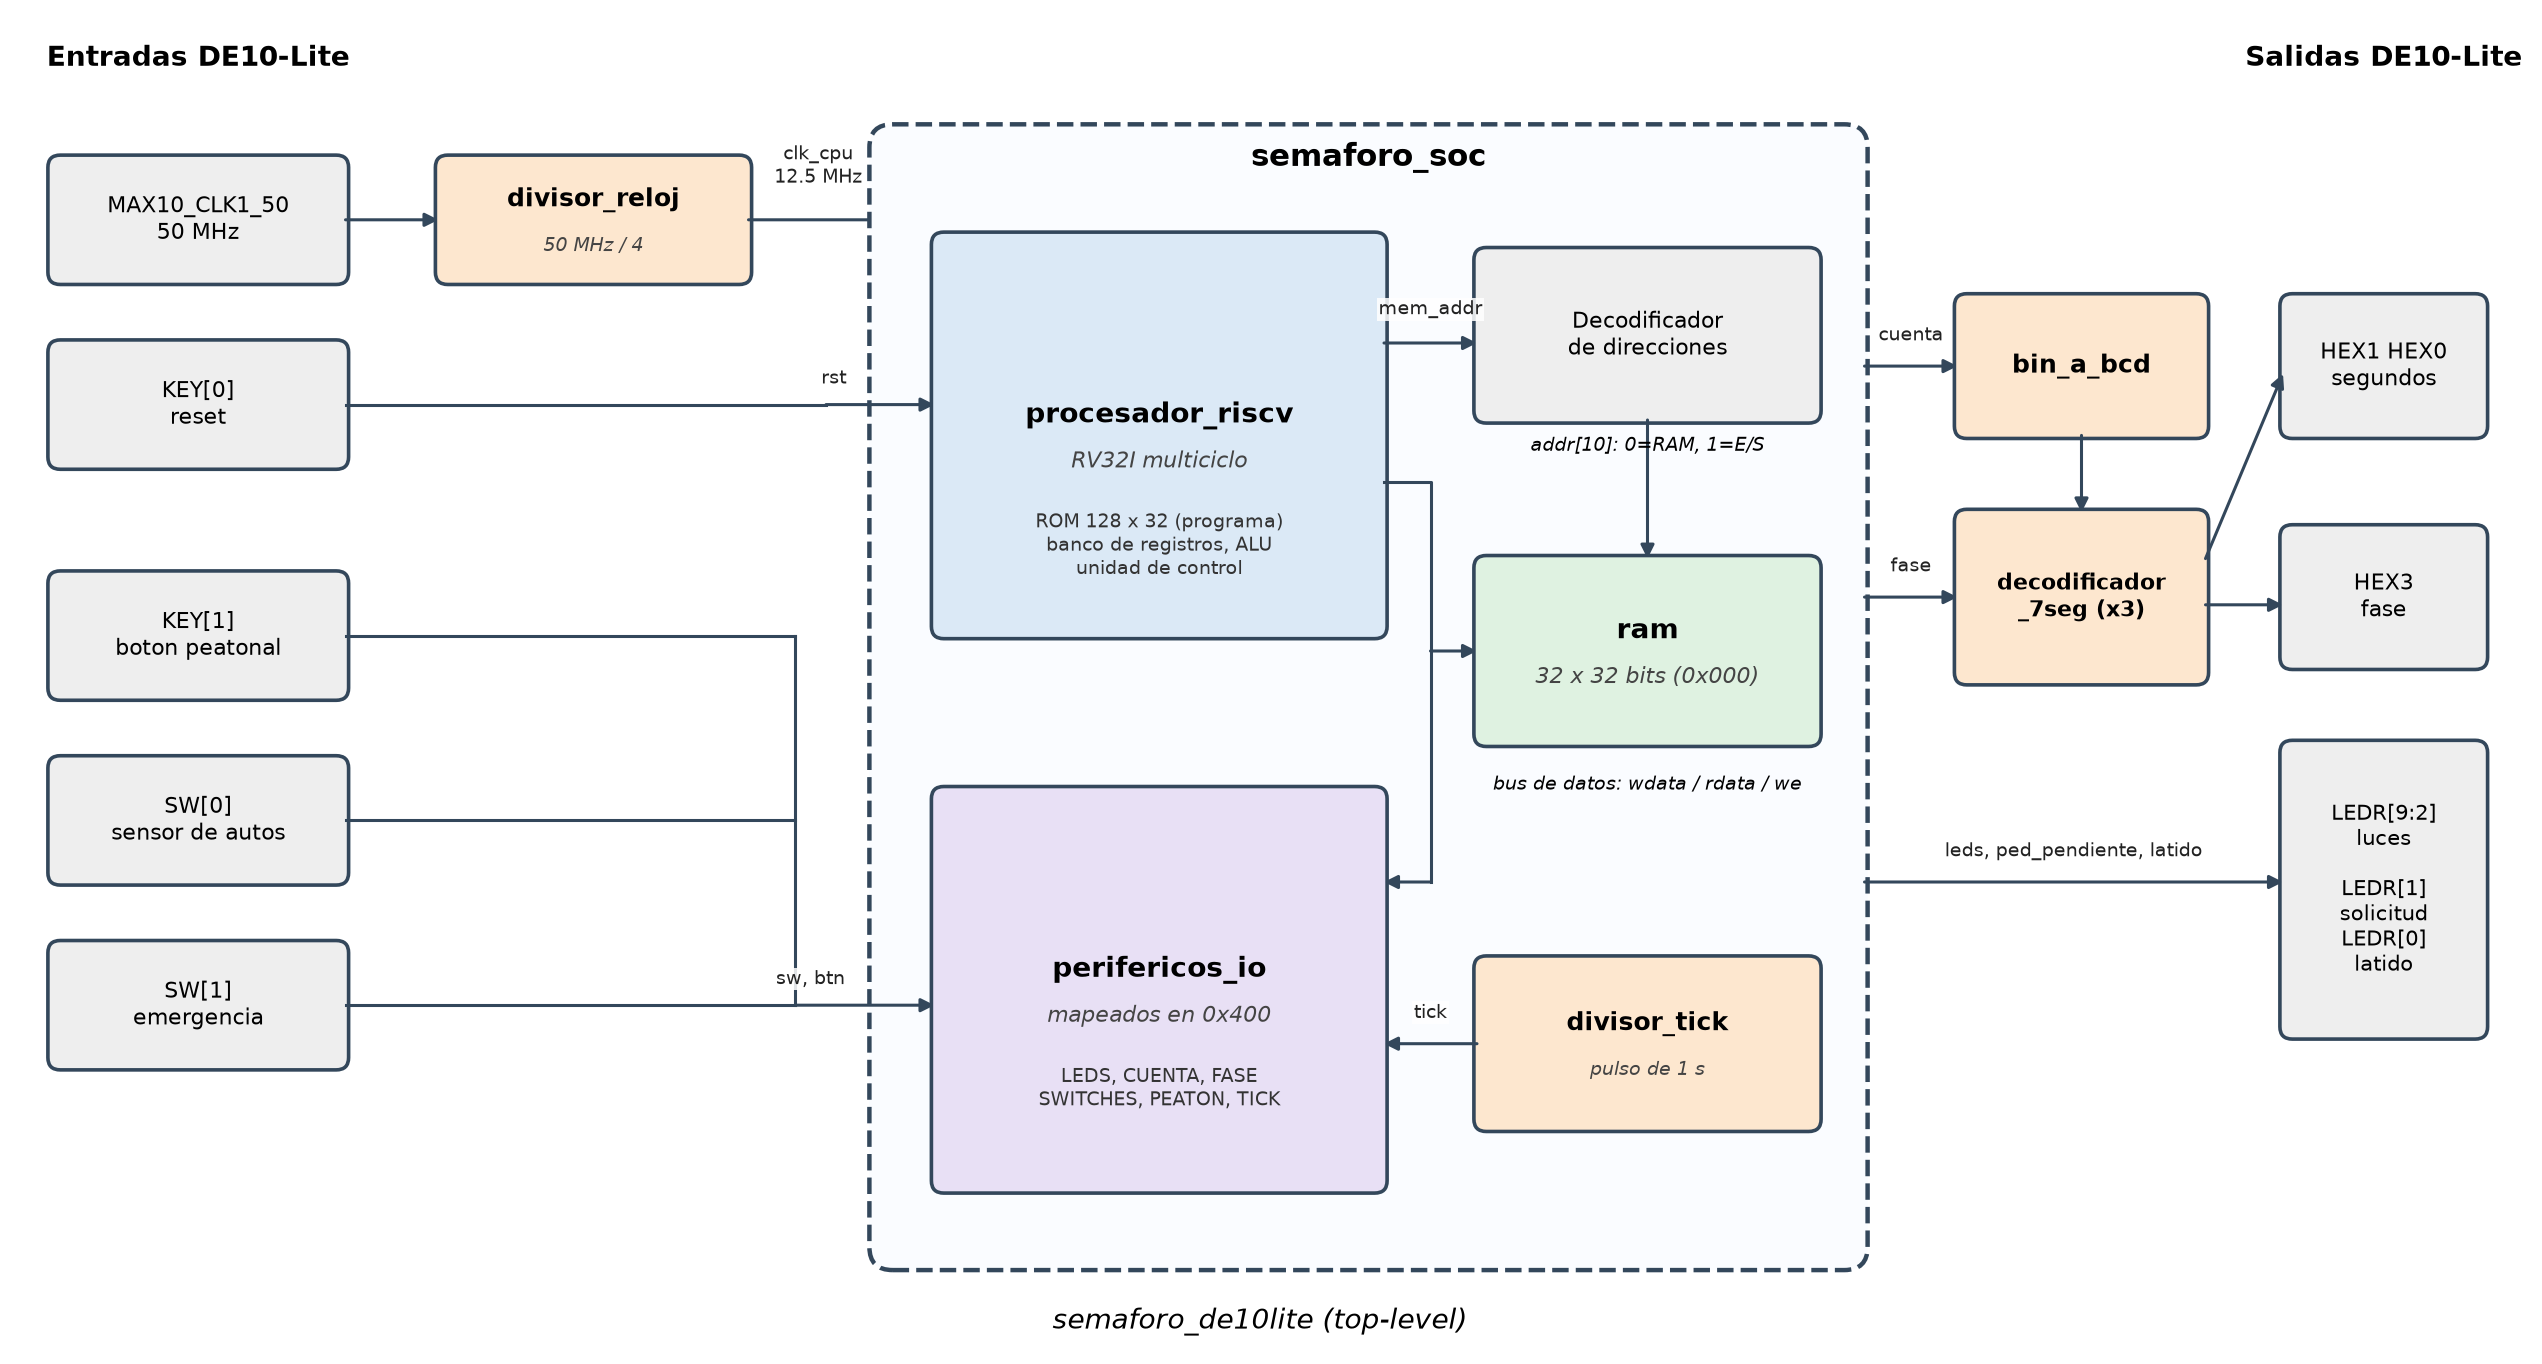
\includegraphics[width=\linewidth]{figuras/diagrama_sistema.png}
  \caption{Diagrama de bloques del sistema completo.}
  \label{fig:sistema}
\end{figure}

La Tabla~\ref{tab:modulos} resume los módulos y su origen. Se marcan como \emph{clase} los que
se usaron sin cambios, como \emph{adaptado} los que se modificaron y como \emph{nuevo} los que
se escribieron para el proyecto.

\begin{table}[H]
  \centering
  \caption{Módulos del proyecto.}
  \label{tab:modulos}
  \small
  \begin{tabular}{llp{8.6cm}}
    \toprule
    Módulo & Origen & Descripción \\
    \midrule
    \cod{alu_riscv} & clase & ALU de 32 bits con operaciones por formato (R, I, B, S, U, J) y banderas. \\
    \cod{adder_nbits} & clase & Sumador parametrizable: calcula PC+4 y PC+inmediato. \\
    \cod{mux_4a1} & clase & Multiplexor 4 a 1 que elige el dato de escritura del banco de registros. \\
    \cod{pipo_register} & clase & Registro PIPO con habilitación: contador de programa (PC). \\
    \cod{rom_file} & adaptado & Memoria de instrucciones (128 palabras); se agregó el parámetro \cod{INIT_FILE}. \\
    \cod{ram} & adaptado & Memoria de datos (32 palabras); se corrigió la polaridad de \cod{we}. \\
    \cod{unidad_control} & adaptado & FSM de \cod{uc_simple} con 2 estados más (saltos) y decodificador de la ALU. \\
    \cod{banco_registros} & nuevo & 32 registros de 32 bits, 2 lecturas y 1 escritura; \cod{x0} = 0. \\
    \cod{generador_inmediatos} & nuevo & Arma el inmediato con signo de los formatos I, S, B, U y J. \\
    \cod{procesador_riscv} & nuevo & Ruta de datos que une todos los bloques anteriores. \\
    \cod{perifericos_io} & nuevo & Registros mapeados en memoria, sincronizadores y detector de flanco. \\
    \cod{divisor_tick} & nuevo & Genera un pulso cada segundo y el latido de \cod{LEDR[0]}. \\
    \cod{divisor_reloj} & nuevo & Divide 50~MHz entre $2^N$ para el procesador. \\
    \cod{bin_a_bcd} & nuevo & Convertidor binario a BCD (\emph{double dabble}). \\
    \cod{decodificador_7seg} & nuevo & Hexadecimal a siete segmentos (ánodo común). \\
    \cod{semaforo_soc} & nuevo & Procesador + RAM + periféricos + decodificador de direcciones. \\
    \cod{semaforo_de10lite} & nuevo & Nivel superior con los pines de la DE10-Lite. \\
    \bottomrule
  \end{tabular}
\end{table}

\subsection{Procesador RISC-V}

\subsubsection{Conjunto de instrucciones soportado}
El procesador ejecuta 25 instrucciones (Tabla~\ref{tab:isa}). Las que usa el programa del
semáforo son \cod{addi}, \cod{andi}, \cod{lw}, \cod{sw}, \cod{beq}, \cod{bne}, \cod{blt},
\cod{jal} y \cod{jalr}. Las demás se agregaron para tener un procesador de propósito general y
se verificaron con el programa de prueba. Cada instrucción se traduce a uno de los
\cod{opcode}/\cod{alu_op} que ya entendía la ALU de clase, así que la ALU se reutilizó sin
cambios.

\begin{table}[H]
  \centering
  \caption{Instrucciones implementadas y operación de la ALU que utilizan.}
  \label{tab:isa}
  \small
  \begin{tabular}{llp{5.2cm}l}
    \toprule
    Formato & Instrucciones & Operación & \cod{alu_op} de \cod{alu_riscv} \\
    \midrule
    R & \cod{add sub and or xor} & $rd \leftarrow rs1 \;op\; rs2$ & \cod{ALU_ADD} \ldots{} \cod{ALU_XOR} \\
    R & \cod{sll srl sra} & corrimientos & \cod{ALU_SLL}, \cod{ALU_SRL}, \cod{ALU_SRA} \\
    R & \cod{slt}, \cod{mul} & comparación con signo, producto & \cod{ALU_I_SLTI}, \cod{ALU_MUL} \\
    I & \cod{addi andi ori xori slti} & $rd \leftarrow rs1 \;op\; imm$ & igual que tipo R \\
    I & \cod{slli srli srai} & corrimiento por \cod{imm[4:0]} & \cod{ALU_SLL} \ldots \\
    I & \cod{lw} & $rd \leftarrow M[rs1+imm]$ & \cod{ALU_I_LW} \\
    I & \cod{jalr} & $rd \leftarrow PC+4;\ PC \leftarrow (rs1+imm)\,\&\,\sim1$ & \cod{ALU_J_JALR} \\
    S & \cod{sw} & $M[rs1+imm] \leftarrow rs2$ & \cod{ALU_S_SW} \\
    B & \cod{beq bne blt} & si se cumple, $PC \leftarrow PC+imm$ & \cod{ALU_B_BEQ/BNE/BLT} \\
    U & \cod{lui} & $rd \leftarrow imm \ll 12$ & \cod{ALU_U_LUI} \\
    J & \cod{jal} & $rd \leftarrow PC+4;\ PC \leftarrow PC+imm$ & (sumador del PC) \\
    \bottomrule
  \end{tabular}
\end{table}

\subsubsection{Ruta de datos}
La Figura~\ref{fig:rutadatos} muestra la ruta de datos (\cod{procesador_riscv.v}). El PC es un
\cod{pipo_register} que solo se actualiza cuando la unidad de control activa \cod{pc_write}. La
dirección de palabra de la ROM es \cod{pc[8:2]}. La instrucción leída alimenta al banco de
registros (campos \cod{rs1}, \cod{rs2} y \cod{rd}), al generador de inmediatos y a la unidad de
control. La entrada B de la ALU se elige entre \cod{rd2} y el inmediato (\cod{alu_src}). El
resultado de la ALU es la dirección del bus de datos, y \cod{rd2} es el dato que se escribe. Un
\cod{mux_4a1} elige qué se escribe en el registro destino: el resultado de la ALU (00), el dato
leído de memoria (01) o PC+4 (10) para \cod{jal}/\cod{jalr}.

Dos instancias de \cod{adder_nbits} calculan PC+4 y PC+inmediato. El siguiente PC es:
\begin{equation*}
  PC_{sig} =
  \begin{cases}
    \text{resultado de la ALU} & \text{si } jalr \\
    PC + imm & \text{si } jump \lor (branch \land \text{ALU}[0]) \\
    PC + 4 & \text{en otro caso}
  \end{cases}
\end{equation*}
En los saltos condicionales la ALU de clase devuelve 1 si se cumple la condición
(\cod{ALU_B_BEQ}, \cod{ALU_B_BNE}, \cod{ALU_B_BLT}), por lo que basta revisar el bit 0 del
resultado.

\begin{figure}[H]
  \centering
  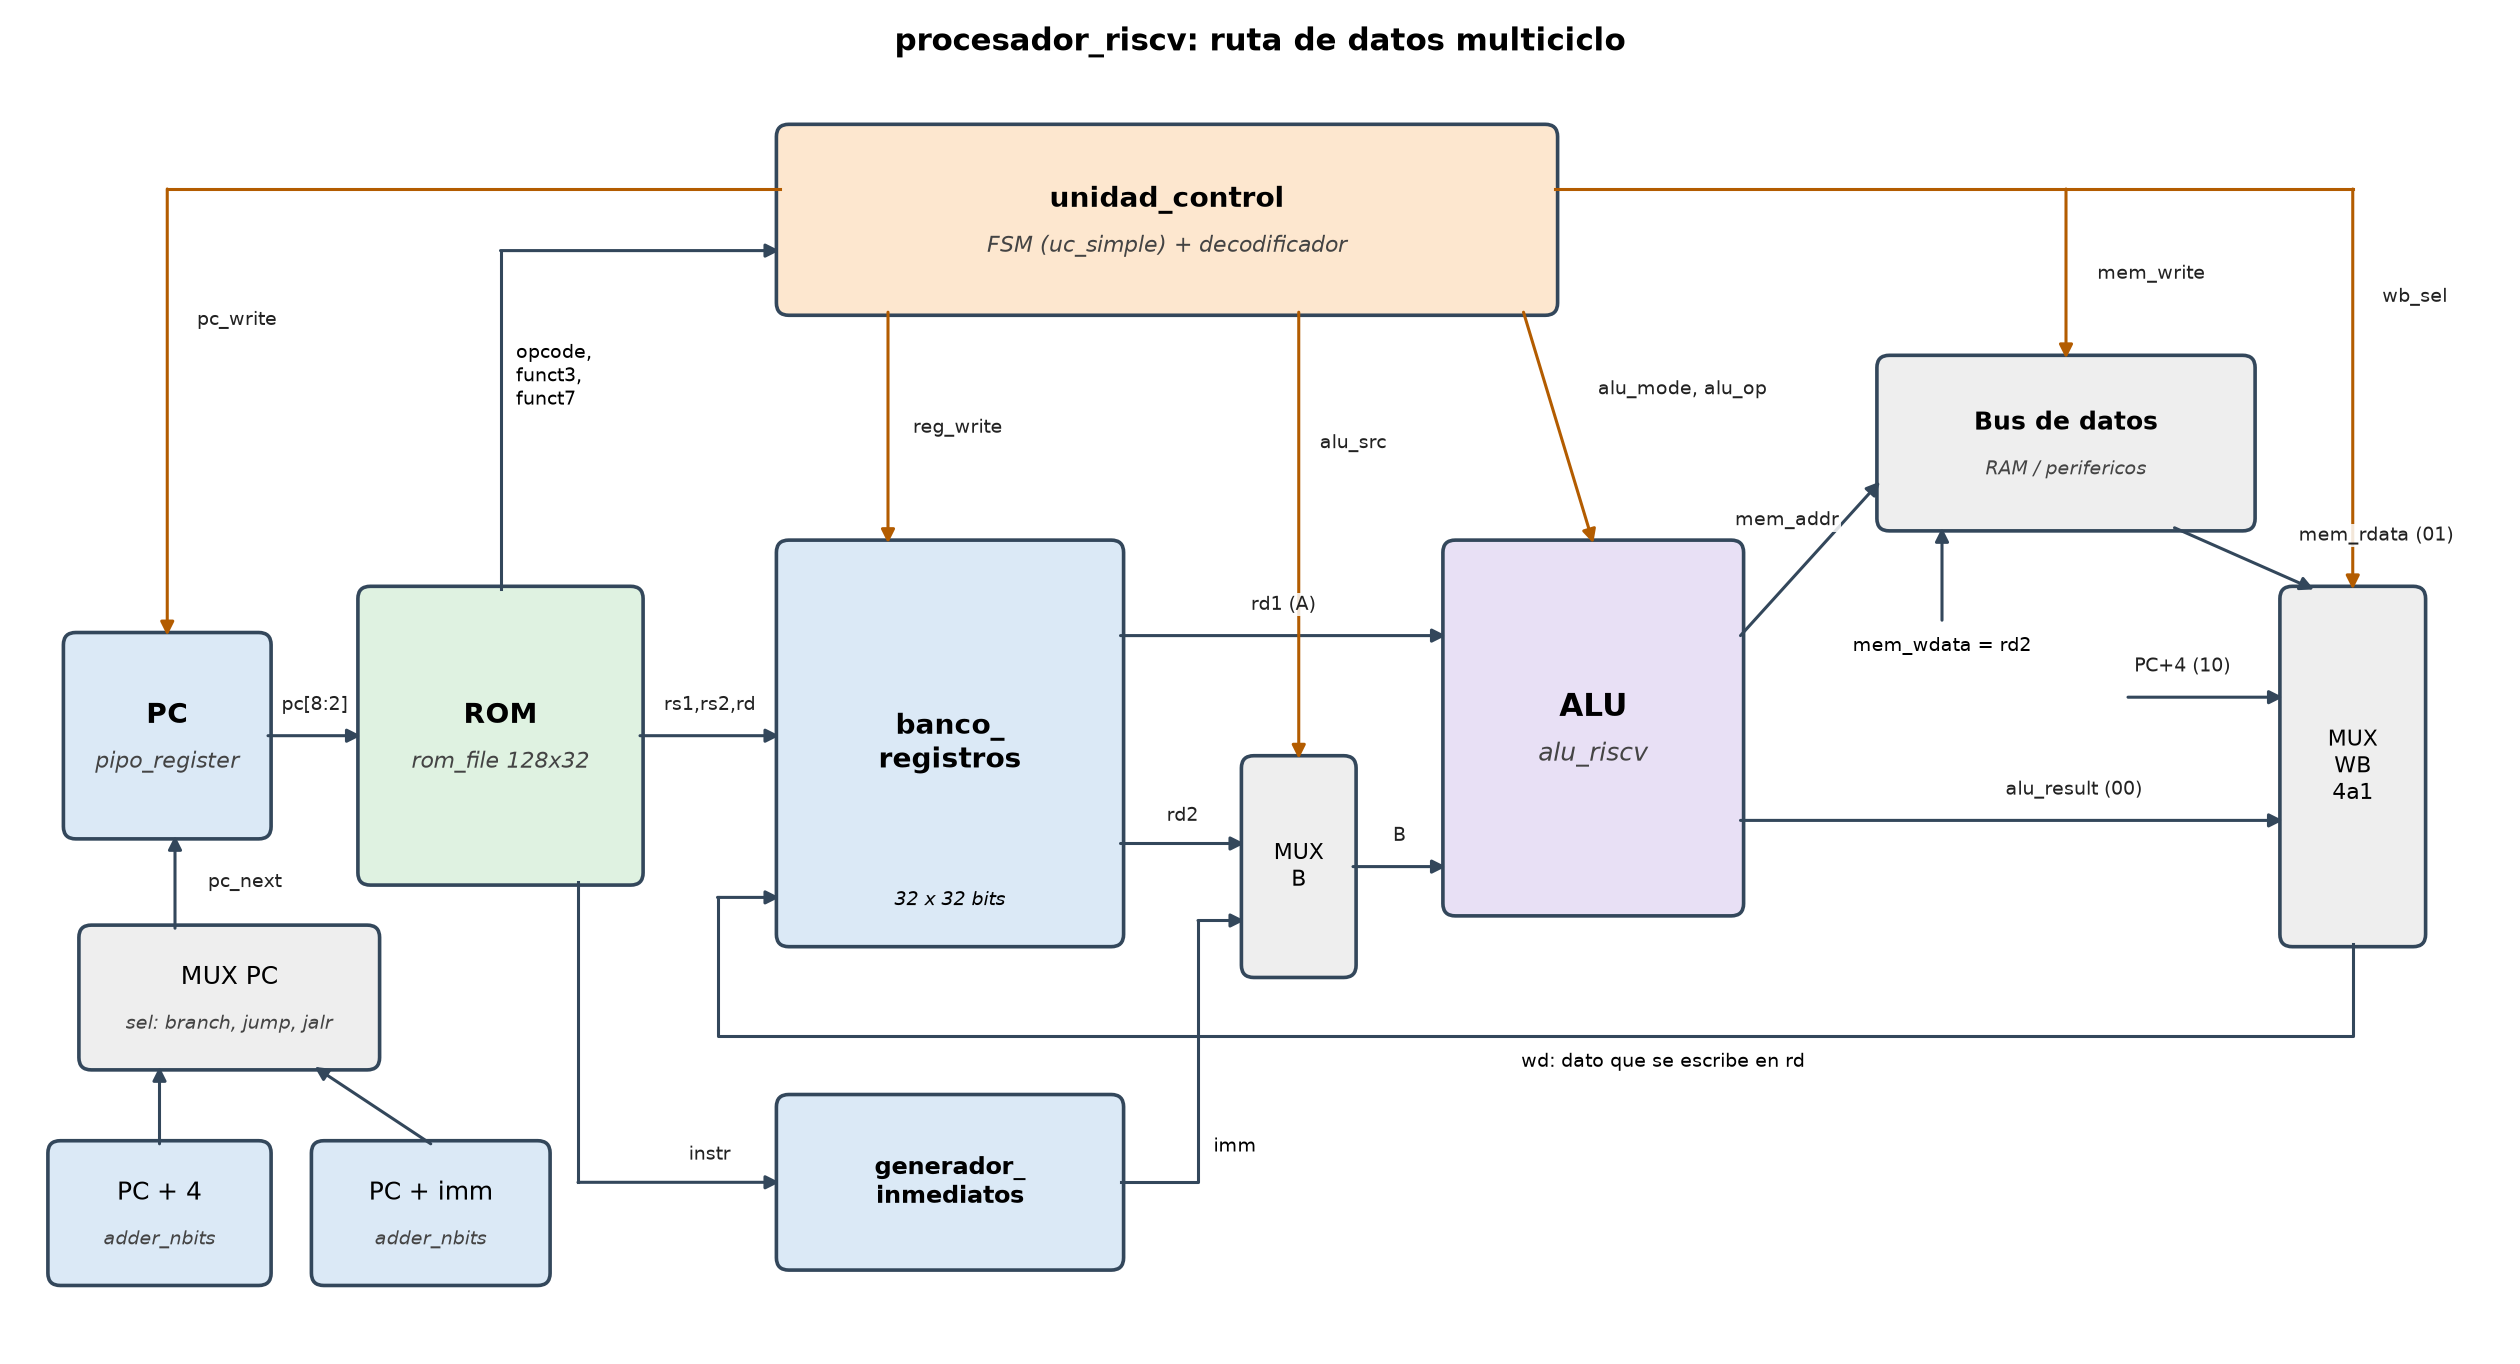
\includegraphics[width=\linewidth]{figuras/diagrama_ruta_datos.png}
  \caption{Ruta de datos del procesador RISC-V multiciclo. En naranja, señales de control.}
  \label{fig:rutadatos}
\end{figure}

\subsubsection{Unidad de control}
La unidad de control (\cod{unidad_control.v}) parte de la máquina de estados \cod{uc_simple} de
clase, con los estados \cod{FETCH}, \cod{DECODE}, \cod{EXEC_R}, \cod{MEM_ADDR},
\cod{MEM_READ}, \cod{MEM_WRITE} y \cod{WRITEBACK}. Se agregaron \cod{EXEC_B} para saltos
condicionales y \cod{EXEC_J} para \cod{jal}/\cod{jalr}, y el registro de estado pasó de 3 a 4
bits. Las salidas de escritura (\cod{pc_write}, \cod{reg_write}, \cod{mem_write}) dependen solo
del estado (estilo Moore). Un decodificador combinacional, que depende de \cod{opcode},
\cod{funct3} y \cod{funct7}, genera \cod{alu_src}, \cod{wb_sel}, \cod{branch}, \cod{jump},
\cod{jalr} y las entradas \cod{opcode}/\cod{alu_op} de la ALU. Una instrucción no reconocida
pasa por \cod{WRITEBACK} sin escribir ningún registro y se comporta como un \cod{nop}.

\begin{figure}[H]
  \centering
  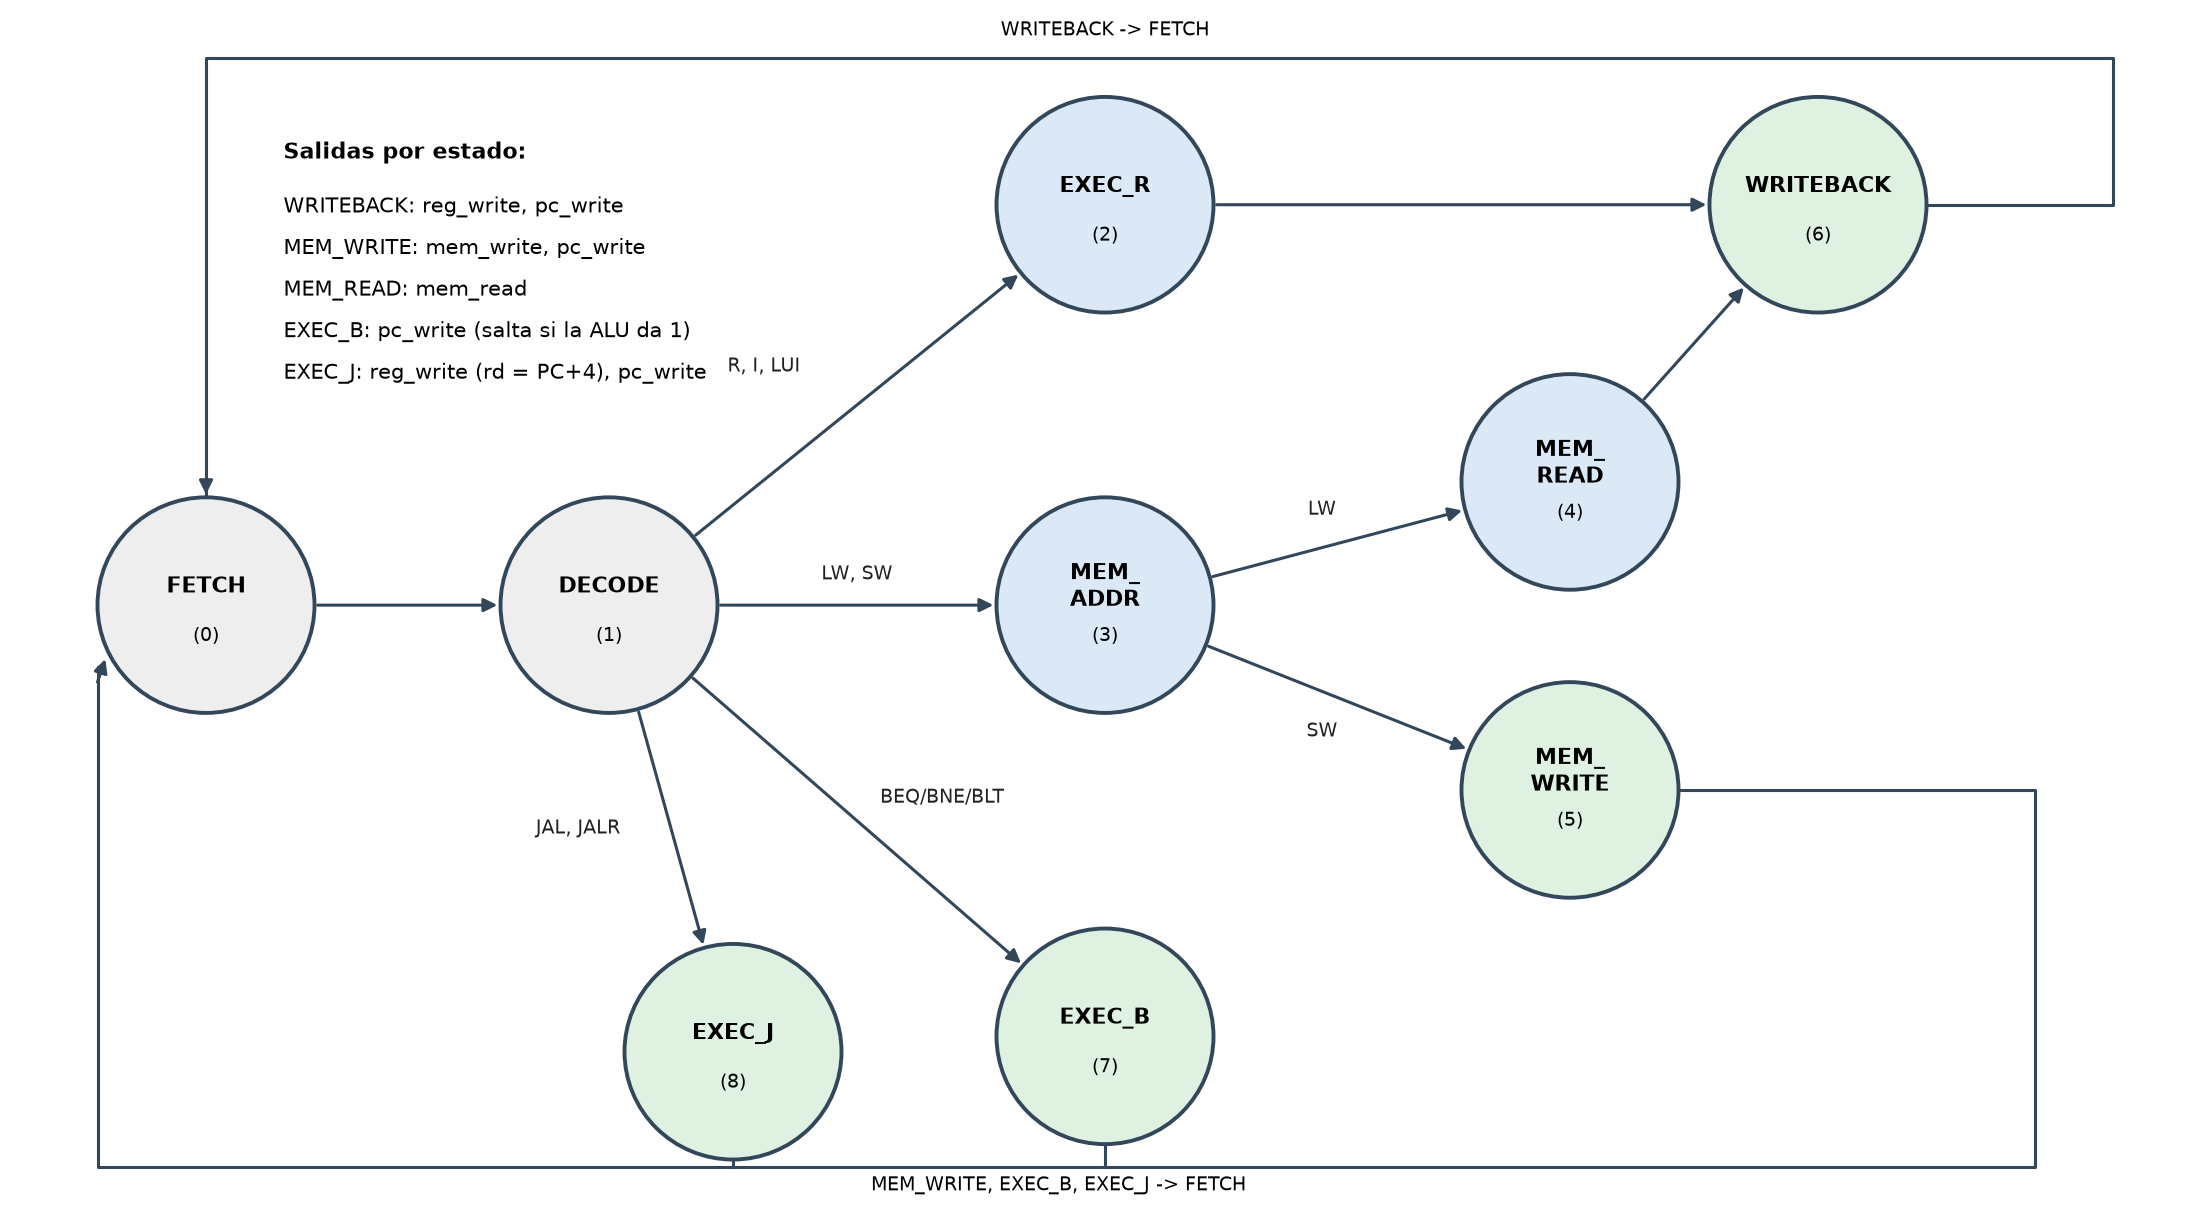
\includegraphics[width=0.95\linewidth]{figuras/diagrama_fsm_control.png}
  \caption{Diagrama de estados de la unidad de control.}
  \label{fig:fsm}
\end{figure}

\begin{table}[H]
  \centering
  \caption{Secuencia de estados y ciclos por instrucción (CPI).}
  \label{tab:cpi}
  \begin{tabular}{llc}
    \toprule
    Tipo de instrucción & Secuencia de estados & Ciclos \\
    \midrule
    R, I, \cod{lui} & FETCH $\rightarrow$ DECODE $\rightarrow$ EXEC\_R $\rightarrow$ WRITEBACK & 4 \\
    \cod{lw} & FETCH $\rightarrow$ DECODE $\rightarrow$ MEM\_ADDR $\rightarrow$ MEM\_READ $\rightarrow$ WRITEBACK & 5 \\
    \cod{sw} & FETCH $\rightarrow$ DECODE $\rightarrow$ MEM\_ADDR $\rightarrow$ MEM\_WRITE & 4 \\
    \cod{beq}, \cod{bne}, \cod{blt} & FETCH $\rightarrow$ DECODE $\rightarrow$ EXEC\_B & 3 \\
    \cod{jal}, \cod{jalr} & FETCH $\rightarrow$ DECODE $\rightarrow$ EXEC\_J & 3 \\
    \bottomrule
  \end{tabular}
\end{table}

Como la ROM es síncrona, el estado \cod{FETCH} sirve para esperar a que la instrucción salga de
la memoria. El PC solo cambia en el último estado de cada instrucción. Por eso la ROM sigue
entregando la misma instrucción durante toda su ejecución y no hace falta un registro de
instrucción adicional.

\subsubsection{Cambios a los módulos de clase}
\begin{itemize}[itemsep=0pt]
  \item \cod{ram.v}: en el código de clase se escribía con \cod{if (!we)}, lo que contradice el
        comentario del propio módulo (\cod{we=1} escritura). Con esa polaridad la RAM se habría
        sobrescrito en cada ciclo de lectura, así que se corrigió a \cod{if (we)}.
  \item \cod{rom_file.v}: se agregó el parámetro \cod{INIT_FILE} para elegir el programa (el
        del semáforo o el de prueba) sin modificar el módulo.
  \item \cod{uc_simple.v} $\rightarrow$ \cod{unidad_control.v}: se agregaron estados, el control
        del PC y el decodificador de la ALU, conservando el mismo estilo de tres bloques
        \cod{always}.
\end{itemize}

\subsection{Mapa de memoria y periféricos}
El bit 10 de la dirección selecciona entre la RAM y los periféricos (Tabla~\ref{tab:mapa}). Así,
el programa puede formar la dirección base \cod{0x400} con una sola instrucción
\cod{addi s0, x0, 1024}. Las entradas de la tarjeta pasan por sincronizadores de dos
\emph{flip-flops}. El botón peatonal se detecta por flanco de bajada y queda guardado en un
registro hasta que el programa lo borra escribiendo en \cod{0x410}. El \emph{tick} de un segundo
funciona igual, por lo que el programa no pierde segundos aunque esté ocupado haciendo otra
cosa.

\begin{table}[H]
  \centering
  \caption{Mapa de memoria del sistema.}
  \label{tab:mapa}
  \small
  \begin{tabular}{llcp{7.4cm}}
    \toprule
    Dirección & Nombre & Acceso & Descripción \\
    \midrule
    \cod{0x000}--\cod{0x07F} & RAM & L/E & 32 palabras. \cod{0x000}: peatones atendidos;
      \cod{0x004}: emergencias; \cod{0x008}: ciclos de la calle. \\
    \cod{0x400} & LEDS & E & Luces del semáforo (\cod{LEDR[9:2]}). \\
    \cod{0x404} & CUENTA & E & Segundos restantes (0--99) para \cod{HEX1}--\cod{HEX0}. \\
    \cod{0x408} & FASE & E & Número de fase para \cod{HEX3}. \\
    \cod{0x40C} & SWITCHES & L & \cod{SW[9:0]} sincronizados (bit 0 autos, bit 1 emergencia). \\
    \cod{0x410} & PEATON & L/E & Lectura: 1 si hay solicitud. Escritura: la borra. \\
    \cod{0x414} & TICK & L/E & Lectura: 1 si pasó un segundo. Escritura: lo borra. \\
    \bottomrule
  \end{tabular}
\end{table}

\subsection{Programa del semáforo}
El programa (\cod{programa_semaforo.asm}, Apéndice~\ref{ap:programas}) tiene 91 instrucciones
(364 bytes) y cabe en la ROM de 128 palabras. Está organizado en una sección por fase y una
subrutina \cod{CUENTA}, que se llama con \cod{jal ra, CUENTA} y regresa con
\cod{jalr x0, 0(ra)}. La subrutina recibe en \cod{s1} el número de segundos y en \cod{s2} un 1
si el botón peatonal puede recortar la fase. En cada vuelta de su ciclo:
\begin{enumerate}[itemsep=0pt]
  \item escribe \cod{s1} en el registro CUENTA (displays);
  \item lee los interruptores y, si \cod{SW[1]} = 1, salta a \cod{EMERGENCIA};
  \item si \cod{s2} = 1, hay solicitud peatonal y quedan más de 3~s, hace \cod{s1} = 3;
  \item si el \emph{tick} está activo, lo borra y decrementa \cod{s1}; regresa cuando \cod{s1} = 0.
\end{enumerate}
Las fases y sus transiciones se muestran en la Figura~\ref{fig:fases} y en la
Tabla~\ref{tab:fases}. El programa también lleva estadísticas en la RAM con \cod{lw}/\cod{sw}.

\begin{figure}[H]
  \centering
  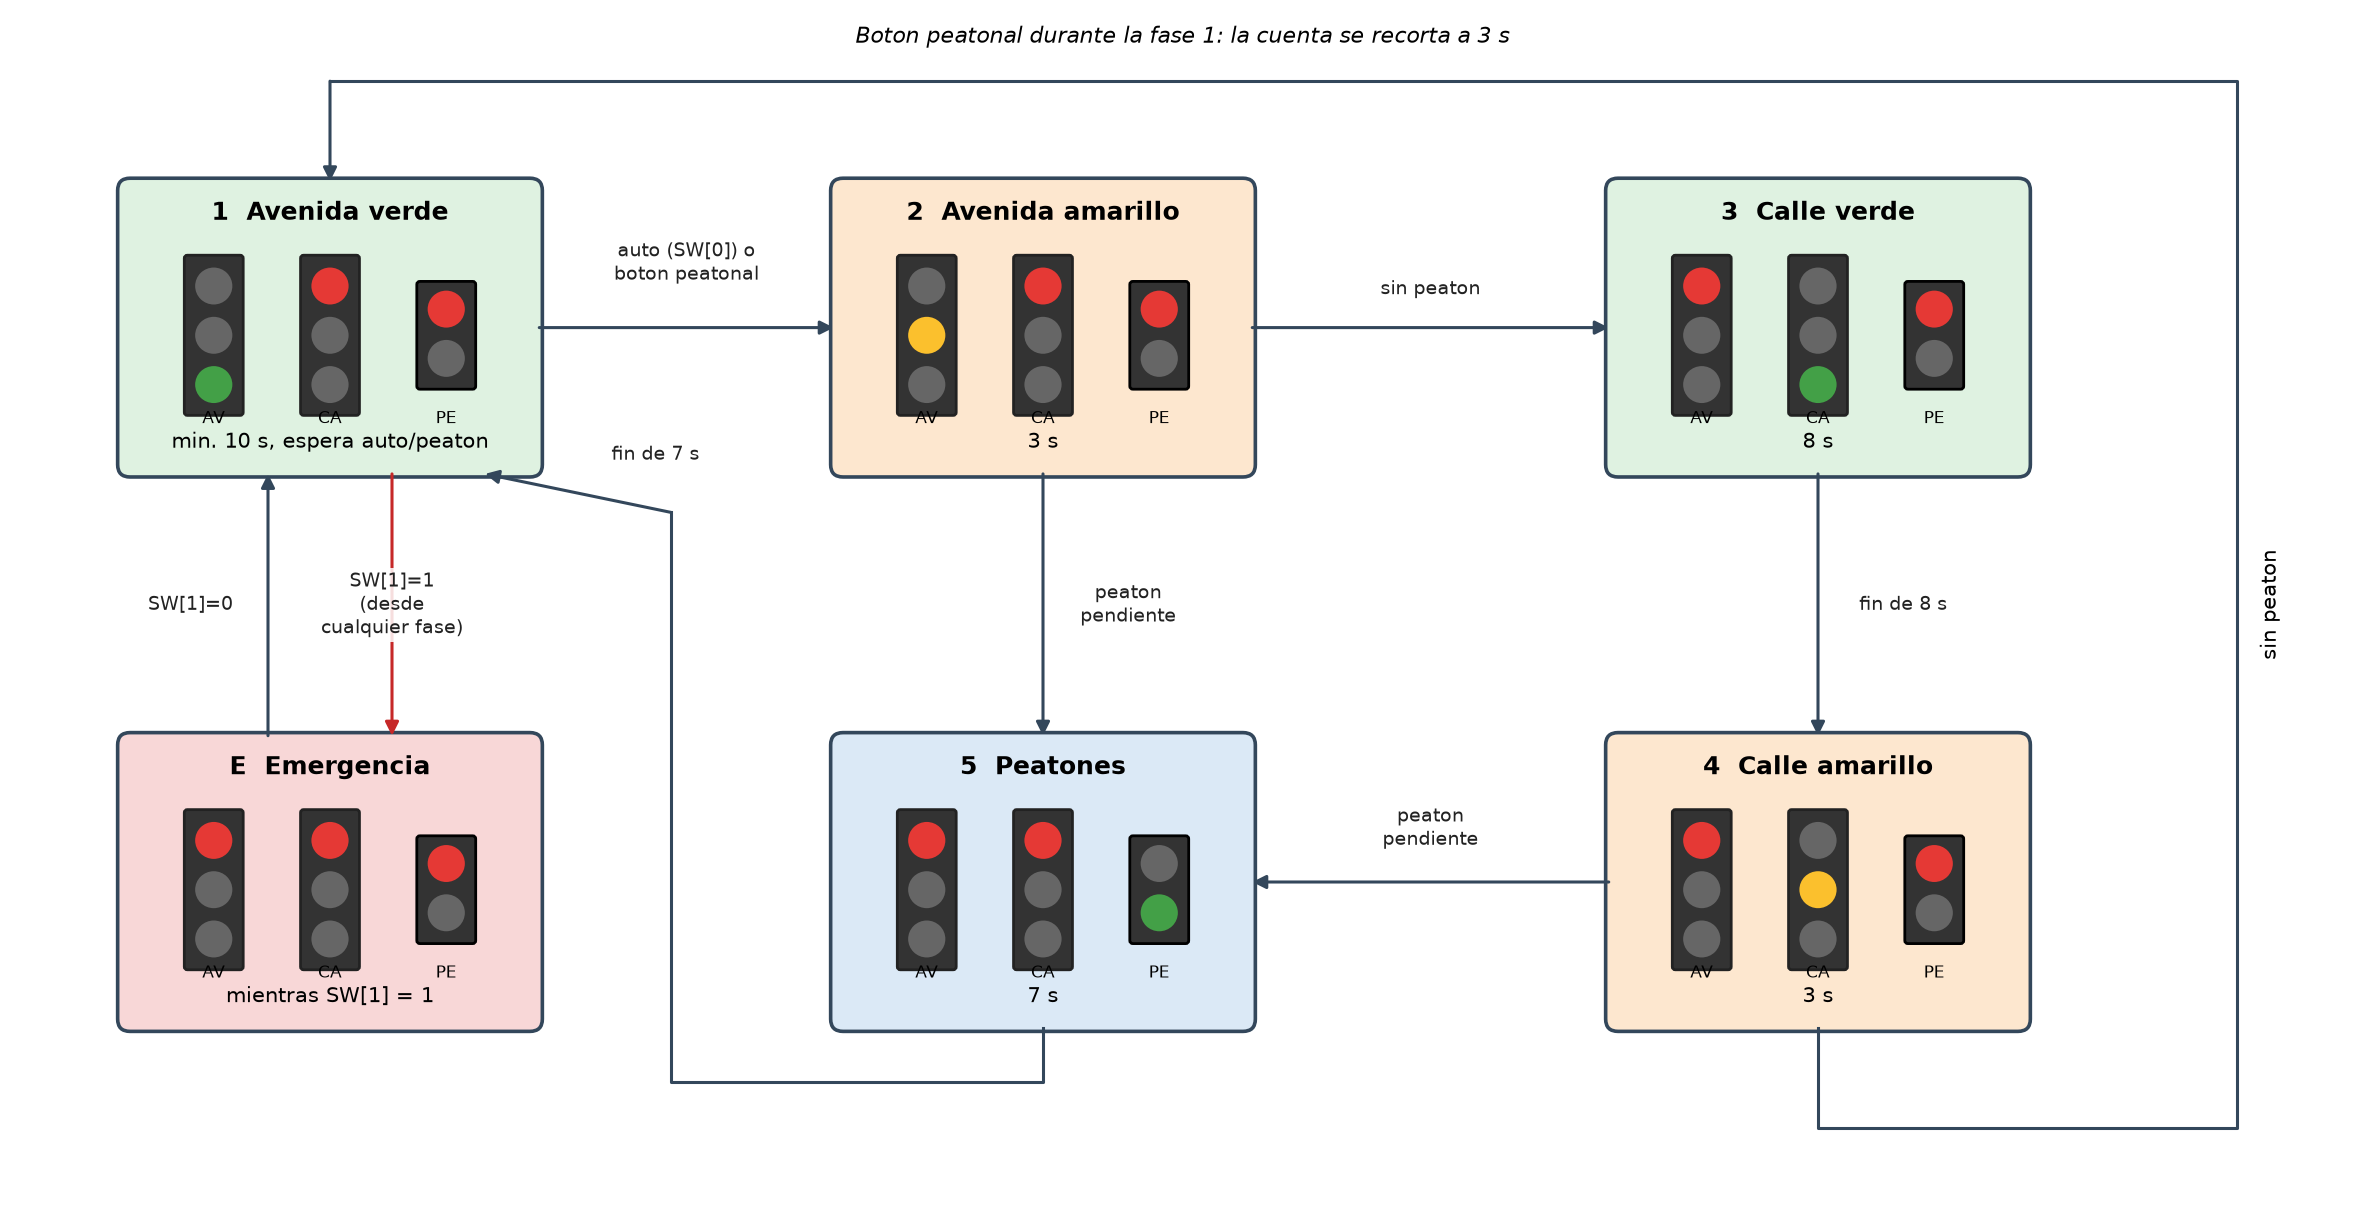
\includegraphics[width=\linewidth]{figuras/diagrama_fases_semaforo.png}
  \caption{Fases del semáforo y condiciones de transición.}
  \label{fig:fases}
\end{figure}

\begin{table}[H]
  \centering
  \caption{Fases del semáforo, luces y valor escrito en el registro LEDS.}
  \label{tab:fases}
  \small
  \begin{tabular}{clcccll}
    \toprule
    Fase & Nombre & AV (R A V) & CA (R A V) & PE (R V) & LEDS & Duración \\
    \midrule
    1 & Avenida verde    & 0 0 1 & 1 0 0 & 1 0 & \cod{0x0C8} & $\geq$ 10 s \\
    2 & Avenida amarillo & 0 1 0 & 1 0 0 & 1 0 & \cod{0x148} & 3 s \\
    3 & Calle verde      & 1 0 0 & 0 0 1 & 1 0 & \cod{0x218} & 8 s \\
    4 & Calle amarillo   & 1 0 0 & 0 1 0 & 1 0 & \cod{0x228} & 3 s \\
    5 & Peatones         & 1 0 0 & 1 0 0 & 0 1 & \cod{0x244} & 7 s \\
    E & Emergencia       & 1 0 0 & 1 0 0 & 1 0 & \cod{0x248} & mientras \cod{SW[1]}=1 \\
    \bottomrule
  \end{tabular}
\end{table}

\subsection{Código máquina del programa}
Cada instrucción del programa se codificó en hexadecimal según su formato (Tabla~\ref{tab:formatos})
y se guardó en \cod{programa_semaforo.hex}, una palabra de 32 bits por línea. La ROM lo carga con
\cod{$readmemh}, igual que \cod{prueba_hex.txt} en el módulo \cod{rom_file} de clase. Las
posiciones que sobran hasta las 128 palabras se rellenan con \cod{nop}. En el
Apéndice~\ref{ap:programas} está el listado con la dirección y el código máquina de cada
instrucción; por ejemplo, \cod{add x3, x1, x2} = \cod{0x002081B3} y
\cod{lui x18, 0x12345} = \cod{0x12345937}.

\subsection{Implementación en la DE10-Lite}
Se preparó un proyecto de Quartus Prime (\cod{quartus/semaforo_de10lite.qpf}) con:
\begin{itemize}[itemsep=0pt]
  \item el dispositivo \cod{10M50DAF484C7G} y \cod{semaforo_de10lite} como entidad superior;
  \item la asignación de los 79 pines usados según el manual de la tarjeta, con estándar
        \cod{3.3-V LVTTL} (Tabla~\ref{tab:pines} y Apéndice~\ref{ap:quartus});
  \item un archivo de restricciones \cod{.sdc} que declara el reloj de 50~MHz y el reloj
        generado de 12.5~MHz, y marca como falsas las rutas de botones, interruptores, LEDs y
        displays.
\end{itemize}
El procesador trabaja a 12.5~MHz (50~MHz entre 4). Así queda un margen amplio para la ruta
combinacional más larga, que va del banco de registros al multiplicador de 32 bits de la ALU y
regresa al banco de registros. Con ese reloj, \cod{TICK_DIV} = 12\,500\,000 ciclos equivale a un
segundo. El archivo \cod{programa_semaforo.hex} debe estar en la carpeta del proyecto de Quartus
para que \cod{$readmemh} lo encuentre durante la síntesis.

\begin{table}[H]
  \centering
  \caption{Asignación de pines principal (DE10-Lite).}
  \label{tab:pines}
  \small
  \begin{tabular}{llll}
    \toprule
    Señal & Pin & Señal & Pin \\
    \midrule
    \cod{MAX10_CLK1_50} & \cod{PIN_P11} & \cod{LEDR[0]} & \cod{PIN_A8} \\
    \cod{KEY[0]} & \cod{PIN_B8} & \cod{LEDR[1]} & \cod{PIN_A9} \\
    \cod{KEY[1]} & \cod{PIN_A7} & \cod{LEDR[2]} & \cod{PIN_A10} \\
    \cod{SW[0]} & \cod{PIN_C10} & \cod{LEDR[3]} & \cod{PIN_B10} \\
    \cod{SW[1]} & \cod{PIN_C11} & \cod{LEDR[4]} & \cod{PIN_D13} \\
    \cod{HEX0[0]} (a) & \cod{PIN_C14} & \cod{LEDR[5]} & \cod{PIN_C13} \\
    \cod{HEX1[0]} (a) & \cod{PIN_C18} & \cod{LEDR[6]} & \cod{PIN_E14} \\
    \cod{HEX3[0]} (a) & \cod{PIN_F21} & \cod{LEDR[7]} & \cod{PIN_D14} \\
    & & \cod{LEDR[8]} & \cod{PIN_A11} \\
    & & \cod{LEDR[9]} & \cod{PIN_B11} \\
    \bottomrule
  \end{tabular}
\end{table}

\noindent\textbf{Procedimiento para programar la tarjeta:}
\begin{enumerate}[itemsep=0pt]
  \item Abrir \cod{quartus/semaforo_de10lite.qpf} en Quartus Prime Lite.
  \item Ejecutar \emph{Processing $\rightarrow$ Start Compilation}.
  \item Conectar la DE10-Lite por USB (USB-Blaster) y abrir \emph{Tools $\rightarrow$ Programmer}.
  \item Seleccionar \cod{output_files/semaforo_de10lite.sof} y presionar \emph{Start}.
  \item Probar: \cod{SW[0]} = autos, \cod{KEY[1]} = peatón, \cod{SW[1]} = emergencia,
        \cod{KEY[0]} = \emph{reset}.
\end{enumerate}

\subsection{Semáforo con LEDs de colores en protoboard}
Los 10 LEDs de la DE10-Lite son rojos, así que en la tarjeta los colores solo se distinguen por
la posición. Por sugerencia del profesor, las luces del semáforo también se sacan por el conector
de expansión GPIO (JP1) hacia LEDs rojos, amarillos y verdes en una protoboard. En
\cod{semaforo_de10lite.v} se agregó el puerto de salida \cod{GPIO[7:0]}, que copia los mismos
bits que el programa escribe en el registro LEDS (\cod{0x400}):
\begin{center}
\cod{assign GPIO = {leds[2], leds[3], leds[4], leds[5], leds[6], leds[7], leds[8], leds[9]};}
\end{center}
No cambió ni el procesador ni el programa: es otra salida para el mismo registro de periférico.
Los 8 LEDs usan los pines 1 a 8 del conector, que están juntos, y la tierra del pin 12
(Figura~\ref{fig:protoboard} y Tabla~\ref{tab:gpio}).

\begin{figure}[H]
  \centering
  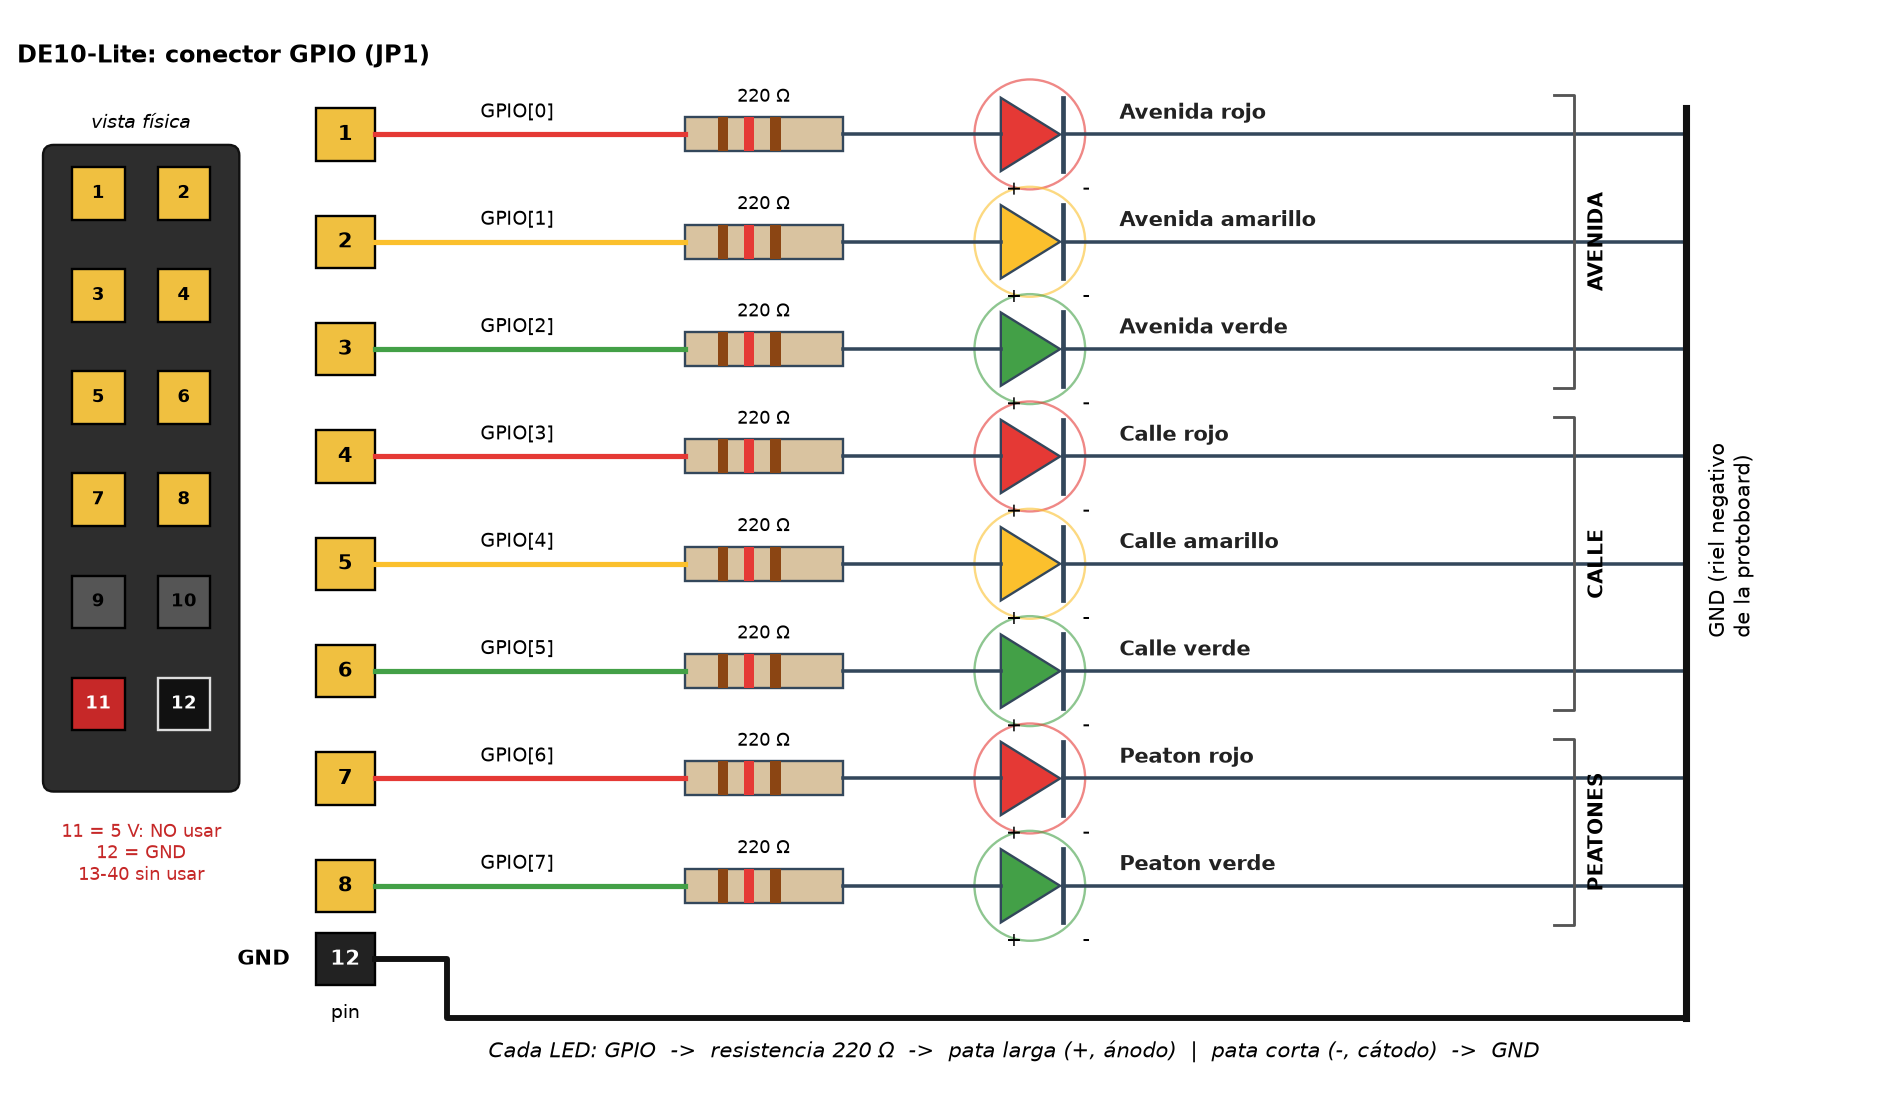
\includegraphics[width=\linewidth]{figuras/diagrama_protoboard.png}
  \caption{Conexión de los LEDs de colores al conector GPIO (JP1) de la DE10-Lite.}
  \label{fig:protoboard}
\end{figure}

\begin{table}[H]
  \centering
  \caption{Asignación de los LEDs de la protoboard.}
  \label{tab:gpio}
  \small
  \begin{tabular}{llccl}
    \toprule
    Señal & Pin FPGA & Pin JP1 & Bit de LEDS & LED \\
    \midrule
    \cod{GPIO[0]} & \cod{PIN_V10} & 1 & 9 & Avenida rojo \\
    \cod{GPIO[1]} & \cod{PIN_W10} & 2 & 8 & Avenida amarillo \\
    \cod{GPIO[2]} & \cod{PIN_V9}  & 3 & 7 & Avenida verde \\
    \cod{GPIO[3]} & \cod{PIN_W9}  & 4 & 6 & Calle rojo \\
    \cod{GPIO[4]} & \cod{PIN_V8}  & 5 & 5 & Calle amarillo \\
    \cod{GPIO[5]} & \cod{PIN_W8}  & 6 & 4 & Calle verde \\
    \cod{GPIO[6]} & \cod{PIN_V7}  & 7 & 3 & Peatón rojo \\
    \cod{GPIO[7]} & \cod{PIN_W7}  & 8 & 2 & Peatón verde \\
    GND & -- & 12 & -- & Cátodo común de los 8 LEDs \\
    \bottomrule
  \end{tabular}
\end{table}

Cada LED se conecta así: pin GPIO $\rightarrow$ resistencia de 220~$\Omega$ $\rightarrow$ ánodo
(pata larga); cátodo (pata corta) $\rightarrow$ GND. La salida es de 3.3~V, así que con un LED
rojo ($V_F \approx 2$~V) la corriente es $I = (3.3 - 2.0)/220 \approx 6$~mA. Es suficiente para
que el LED se vea encendido y no excede la corriente que entrega un pin del MAX~10 con el
estándar \cod{3.3-V LVTTL}. El pin 11 del conector (5~V) no se usa.

\subsection{Estrategia de verificación}
Cada \emph{testbench} se escribió con el mismo estilo que en clase (declaración de señales,
instanciación de la UUT y bloque de estímulos). Además compara automáticamente las salidas
contra los valores esperados, cuenta los errores y escribe los resultados en la consola y en un
archivo \cod{resultados_*.txt}. Para que la simulación del sistema sea corta, el
\emph{testbench} cambia el parámetro \cod{TICK_DIV} a 200, así que un ``segundo'' dura
$200 \times 80\text{ ns} = 16~\mu\text{s}$. La lógica del semáforo es la misma, solo que más
rápida. Las simulaciones se ejecutaron en Active-HDL~\cite{aldec}: se compilan todos los
archivos del diseño, se elige el \emph{testbench} como unidad superior, se agregan las señales
al visor de formas de onda y se corre la simulación hasta \cod{$finish}.

\begin{table}[H]
  \centering
  \caption{Bancos de prueba desarrollados.}
  \label{tab:tbs}
  \small
  \begin{tabular}{lp{10.5cm}}
    \toprule
    \emph{Testbench} & Qué verifica \\
    \midrule
    \cod{tb_banco_registros} & \emph{Reset}, escritura/lectura, que \cod{x0} no se escriba,
      lectura doble simultánea y que no se escriba con \cod{we}=0. \\
    \cod{tb_perifericos_io} & Escritura de LEDS/CUENTA/FASE, lectura sincronizada de los
      interruptores, guardado y borrado de la solicitud peatonal y del \emph{tick}. \\
    \cod{tb_procesador_riscv} & Ejecuta \cod{prueba_instrucciones.asm} (todas las instrucciones,
      saltos tomados y no tomados, subrutina y ciclo) y compara 25 registros y 2 palabras de RAM. \\
    \cod{tb_semaforo_de10lite} & Sistema completo desde los pines: arranque, avenida en espera,
      sensor de autos, botón peatonal con recorte, emergencia, displays y estadísticas en RAM. \\
    \bottomrule
  \end{tabular}
\end{table}

% =====================================================================
\section{Resultados}\label{sec:resultados}
% =====================================================================
Todos los módulos compilaron en Active-HDL sin errores ni advertencias, y los cuatro
\emph{testbenches} terminaron con el mensaje ``TODAS LAS PRUEBAS PASARON''. Los registros de
consola completos están en el Apéndice~\ref{ap:logs}.

\subsection{Banco de registros}
En la Figura~\ref{fig:wbanco} se escriben \cod{0x0000000F}, \cod{0xDEADBEEF} y \cod{0xFFFFFFFF}
en \cod{x1}, \cod{x2} y \cod{x31}. Después se intenta escribir \cod{0x12345678} en \cod{x0}, y la
lectura sigue en cero. Las 9 verificaciones pasaron.
\begin{figure}[H]
  \centering
  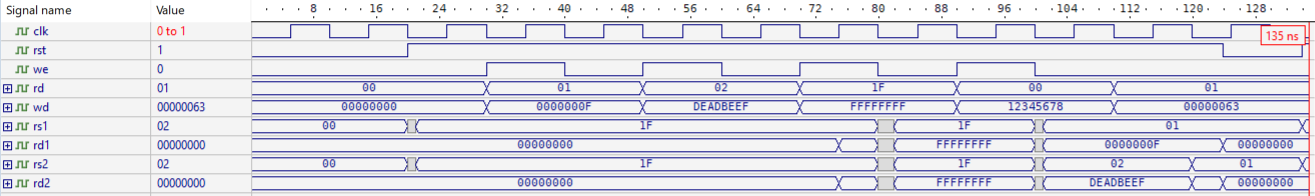
\includegraphics[width=\linewidth]{figuras/wave_banco_registros.png}
  \caption{Simulación del banco de registros.}
  \label{fig:wbanco}
\end{figure}

\subsection{Periféricos mapeados en memoria}
En la Figura~\ref{fig:wperif} se observa que los registros LEDS (\cod{0x0C8}), CUENTA (10) y
FASE (1) toman el valor escrito, y que los interruptores (\cod{0000000011}) se leen dos ciclos
después de cambiar, por el sincronizador. El pulso del botón activa \cod{ped_pendiente}, que
se mantiene hasta la escritura en el registro 4; el \emph{tick} se comporta igual con el
registro 5. Las 8 verificaciones pasaron.
\begin{figure}[H]
  \centering
  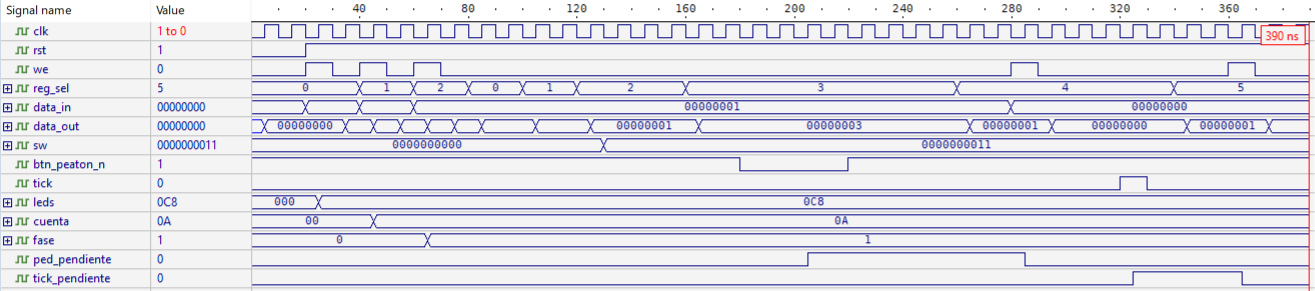
\includegraphics[width=\linewidth]{figuras/wave_perifericos.png}
  \caption{Simulación de los periféricos.}
  \label{fig:wperif}
\end{figure}

\subsection{Procesador RISC-V}
La Figura~\ref{fig:wfsm} muestra las primeras instrucciones del programa de prueba. Se ve la
secuencia de estados \texttt{0}$\rightarrow$\texttt{1}$\rightarrow$\texttt{2}$\rightarrow$\texttt{6}
(FETCH, DECODE, EXEC\_R, WRITEBACK) de las instrucciones tipo R e I, con \cod{reg_write} y
\cod{pc_write} activos solo en WRITEBACK, y el PC avanzando de 4 en 4. En la
Figura~\ref{fig:wsaltos} aparecen \cod{sw} (estados 3$\rightarrow$5 con \cod{mem_we}=1),
\cod{lw} (3$\rightarrow$4$\rightarrow$6), los saltos condicionales (estado 7) y la llamada a la
subrutina (estado 8): el PC salta de \cod{0x6C} a \cod{0x90} y regresa a \cod{0x70}. La
Figura~\ref{fig:wproc} muestra la ejecución completa: \cod{x23} acumula 5, 9, 12, 14 y 15 en el
ciclo. La Tabla~\ref{tab:regs} compara los registros finales con los valores esperados.

\begin{figure}[H]
  \centering
  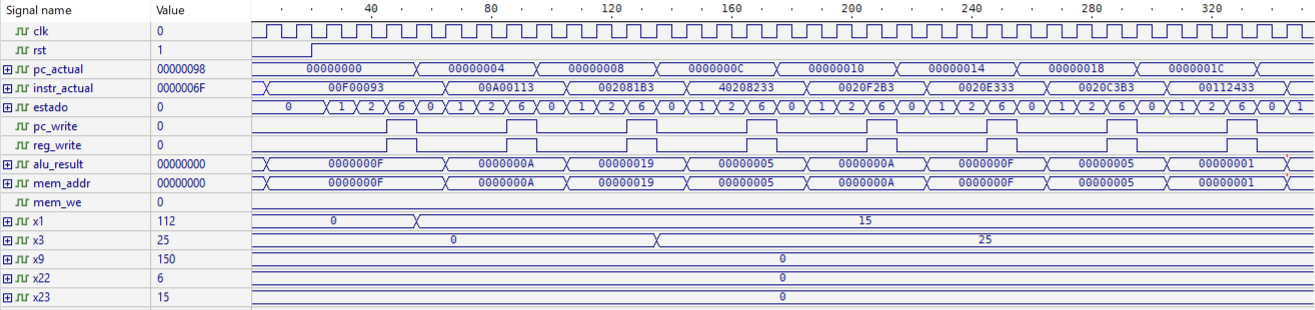
\includegraphics[width=\linewidth]{figuras/wave_procesador_fsm.png}
  \caption{Procesador: primeras instrucciones (tipo R) y estados de la unidad de control.}
  \label{fig:wfsm}
\end{figure}

\begin{figure}[H]
  \centering
  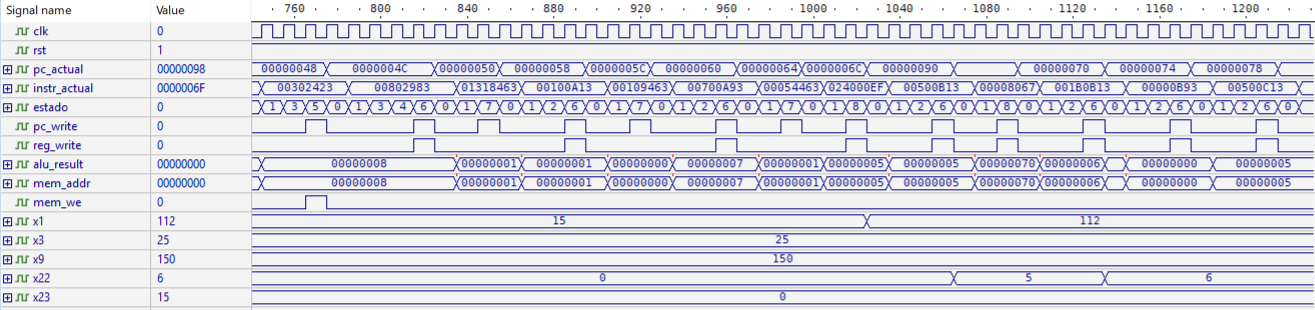
\includegraphics[width=\linewidth]{figuras/wave_procesador_saltos.png}
  \caption{Procesador: \cod{sw}, \cod{lw}, saltos condicionales, \cod{jal} y \cod{jalr}.}
  \label{fig:wsaltos}
\end{figure}

\begin{figure}[H]
  \centering
  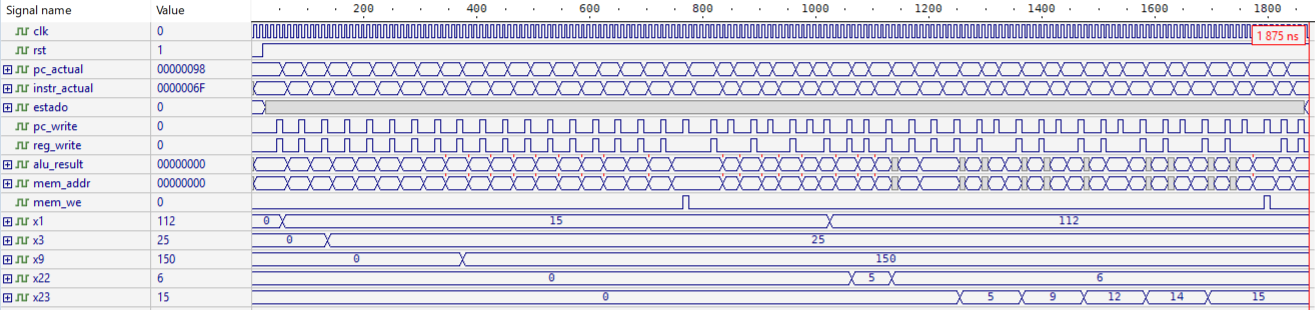
\includegraphics[width=\linewidth]{figuras/wave_procesador_completo.png}
  \caption{Procesador: ejecución completa del programa de prueba (1.875~$\mu$s).}
  \label{fig:wproc}
\end{figure}

\begin{table}[H]
  \centering
  \caption{Resultado del programa de prueba de instrucciones.}
  \label{tab:regs}
  \small
  \begin{tabular}{lllll}
    \toprule
    Registro & Instrucción probada & Esperado & Obtenido & \\
    \midrule
    \cod{x1}  & \cod{jal x1} (dir. de regreso) & \cod{0x00000070} & \cod{0x00000070} & OK \\
    \cod{x3}  & \cod{add}  & 25 & 25 & OK \\
    \cod{x4}  & \cod{sub}  & 5 & 5 & OK \\
    \cod{x5}  & \cod{and}  & 10 & 10 & OK \\
    \cod{x6}  & \cod{or}   & 15 & 15 & OK \\
    \cod{x7}  & \cod{xor}  & 5 & 5 & OK \\
    \cod{x8}  & \cod{slt}  & 1 & 1 & OK \\
    \cod{x9}  & \cod{mul}  & 150 & 150 & OK \\
    \cod{x10} & \cod{addi} negativo & $-3$ & $-3$ & OK \\
    \cod{x11} & \cod{slti} & 1 & 1 & OK \\
    \cod{x12} & \cod{slli} & 240 & 240 & OK \\
    \cod{x13} & \cod{srai} & $-2$ & $-2$ & OK \\
    \cod{x14} & \cod{srli} & 60 & 60 & OK \\
    \cod{x15} & \cod{andi} & 6 & 6 & OK \\
    \cod{x16} & \cod{ori}  & 15 & 15 & OK \\
    \cod{x17} & \cod{xori} & 240 & 240 & OK \\
    \cod{x18} & \cod{lui}  & \cod{0x12345000} & \cod{0x12345000} & OK \\
    \cod{x19} & \cod{sw} + \cod{lw} & 25 & 25 & OK \\
    \cod{x20} & \cod{beq} tomado & 1 & 1 & OK \\
    \cod{x21} & \cod{bne} no tomado, \cod{blt} tomado & 7 & 7 & OK \\
    \cod{x22} & \cod{jal} / \cod{jalr} & 6 & 6 & OK \\
    \cod{x23} & ciclo con \cod{bne} & 15 & 15 & OK \\
    \cod{x0}  & no escribible & 0 & 0 & OK \\
    RAM[2], RAM[3] & \cod{sw} & 25, 15 & 25, 15 & OK \\
    \bottomrule
  \end{tabular}
\end{table}

El programa llegó a la etiqueta \cod{FIN} en 184 ciclos y se decodificaron 49 instrucciones.

\subsection{Sistema completo: semáforo inteligente}
La Figura~\ref{fig:wsem} muestra la simulación completa del sistema (845~$\mu$s, equivalentes a
unos 53 segundos reales). Las señales \cod{avenida}, \cod{calle} y \cod{peaton} están en el
orden (rojo, amarillo, verde) y (rojo, verde), así que \cod{001} significa verde y \cod{100}
rojo. En las Figuras~\ref{fig:warr} a~\ref{fig:wemer} se amplía cada escenario y la
Tabla~\ref{tab:escenarios} resume las verificaciones.

\begin{figure}[H]
  \centering
  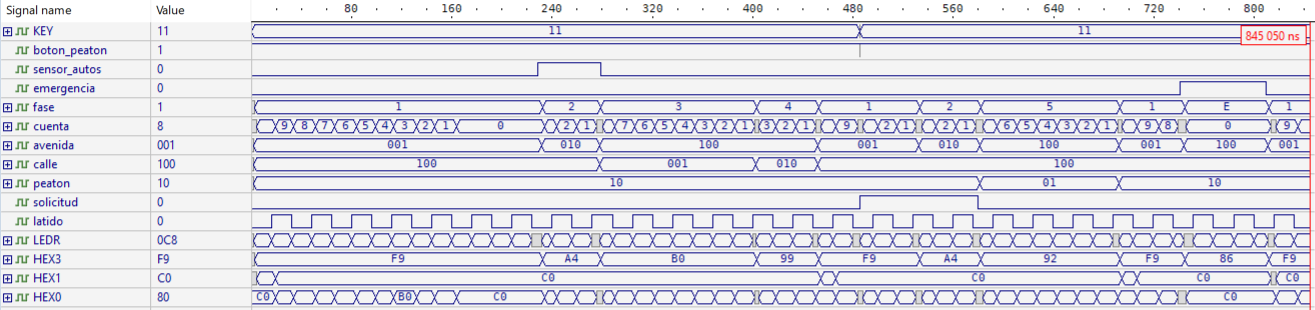
\includegraphics[width=\linewidth]{figuras/wave_semaforo_completo.png}
  \caption{Simulación completa del semáforo inteligente.}
  \label{fig:wsem}
\end{figure}

\begin{figure}[H]
  \centering
  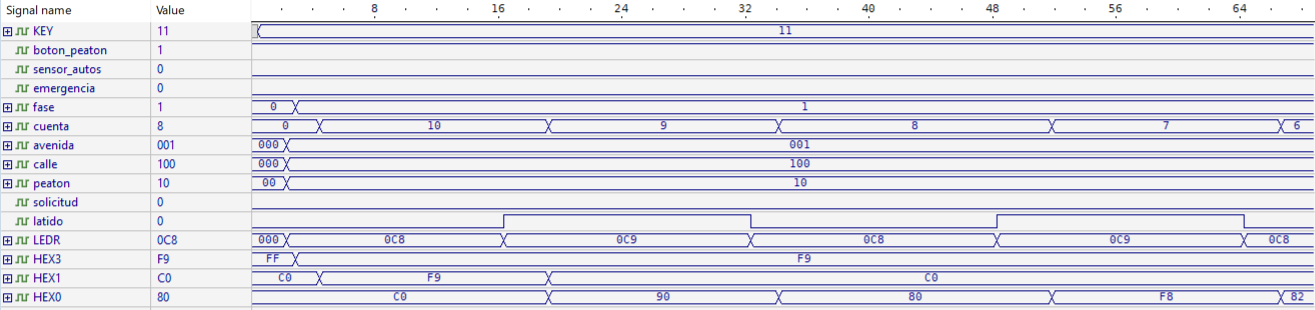
\includegraphics[width=\linewidth]{figuras/wave_semaforo_arranque.png}
  \caption{Arranque: después del \emph{reset} el programa enciende la fase 1 y la cuenta baja
  de 10 a 0 con cada \emph{tick} (\cod{latido}).}
  \label{fig:warr}
\end{figure}

\begin{figure}[H]
  \centering
  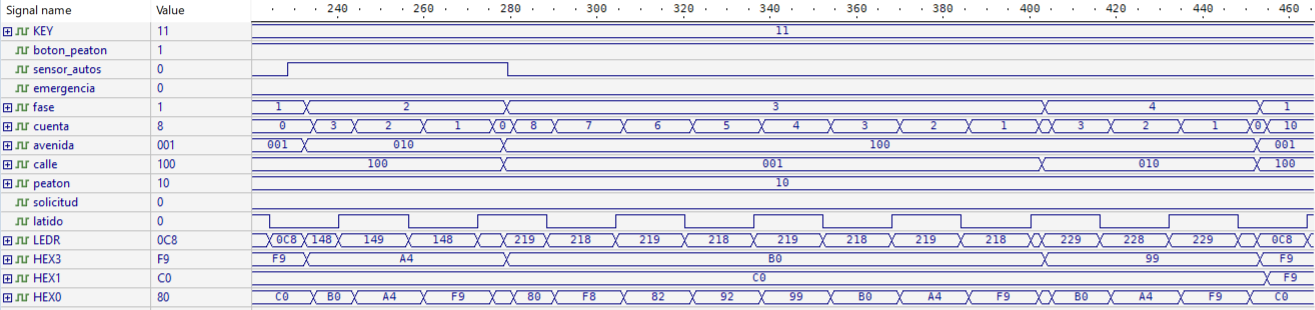
\includegraphics[width=\linewidth]{figuras/wave_semaforo_autos.png}
  \caption{Sensor de autos: al activar \cod{SW[0]} la avenida pasa a amarillo (fase 2, 3~s),
  la calle recibe verde (fase 3, 8~s) y amarillo (fase 4, 3~s), y regresa a la fase 1.}
  \label{fig:wautos}
\end{figure}

\begin{figure}[H]
  \centering
  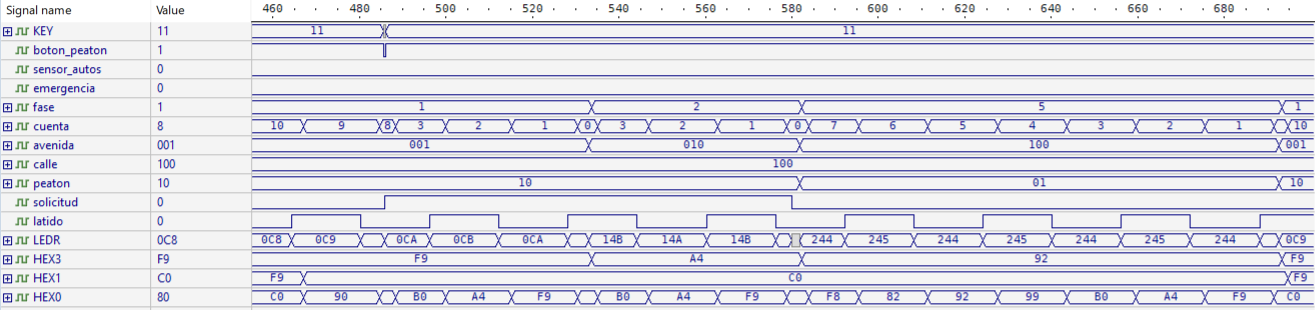
\includegraphics[width=\linewidth]{figuras/wave_semaforo_peaton.png}
  \caption{Botón peatonal: el pulso en \cod{KEY[1]} activa \cod{solicitud}; la cuenta de la
  avenida se recorta de 8 a 3, luego vienen el amarillo y la fase 5 con el peatón en verde
  (\cod{peaton} = \cod{01}). La solicitud se borra al atenderla.}
  \label{fig:wpeat}
\end{figure}

\begin{figure}[H]
  \centering
  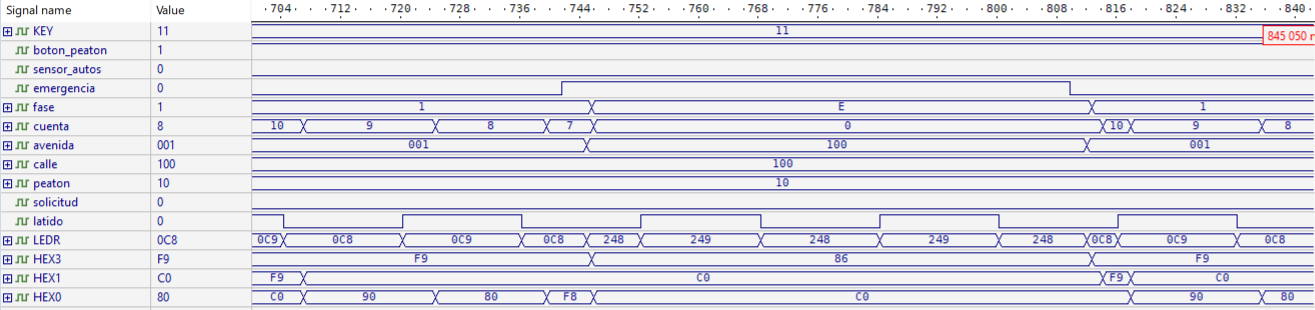
\includegraphics[width=\linewidth]{figuras/wave_semaforo_emergencia.png}
  \caption{Emergencia: al activar \cod{SW[1]} la fase cambia a \texttt{E}, todos los semáforos
  quedan en rojo y la cuenta en 0; al desactivarlo se reinicia la fase 1 con 10~s.}
  \label{fig:wemer}
\end{figure}

\begin{figure}[H]
  \centering
  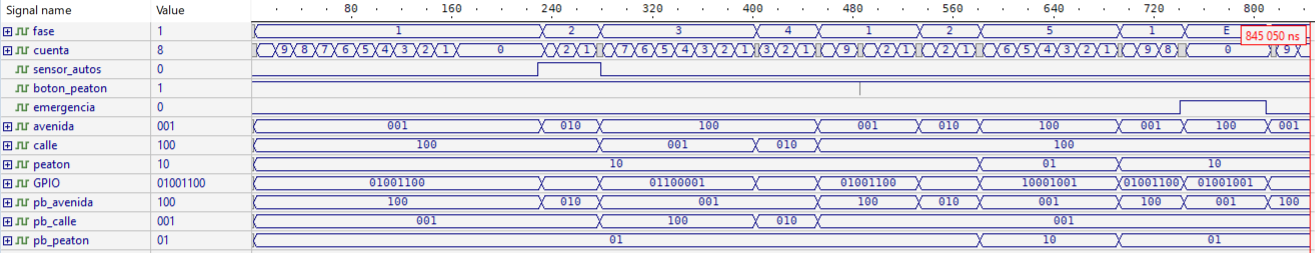
\includegraphics[width=\linewidth]{figuras/wave_semaforo_protoboard.png}
  \caption{Salidas hacia la protoboard: \cod{GPIO} repite las luces de \cod{avenida},
  \cod{calle} y \cod{peaton}. \cod{pb_avenida} = \cod{GPIO[2:0]} se lee como (verde, amarillo,
  rojo), en orden inverso a \cod{LEDR}.}
  \label{fig:wgpio}
\end{figure}

\begin{table}[H]
  \centering
  \caption{Escenarios verificados en \cod{tb_semaforo_de10lite}.}
  \label{tab:escenarios}
  \small
  \begin{tabular}{p{3.3cm}p{8.6cm}c}
    \toprule
    Escenario & Verificación & Resultado \\
    \midrule
    1. Arranque & Fase 1, luces AV verde / CA rojo / PE rojo; \cod{HEX1 HEX0} = ``10'';
      \cod{HEX3} = ``1''. & OK \\
    2. Sin autos & Después de 14~s la avenida sigue en verde con cuenta 0. & OK \\
    3. Sensor de autos & Fases 2 $\rightarrow$ 3 $\rightarrow$ 4 $\rightarrow$ 1 con las luces correctas. & OK \\
    4. Botón peatonal & \cod{LEDR[1]}=1, recorte a $\leq$3~s, fases 2 $\rightarrow$ 5 $\rightarrow$ 1;
      la solicitud se borra. & OK \\
    5. Emergencia & Fase E, todo en rojo, \cod{HEX3} = ``E''; se mantiene mientras \cod{SW[1]}=1;
      regresa a fase 1. & OK \\
    6. Estadísticas & RAM[0] = 1 peatón, RAM[1] = 1 emergencia, RAM[2] = 1 ciclo de la calle. & OK \\
    7. Protoboard & En las 10 revisiones de luces, \cod{GPIO[7:0]} coincide con \cod{LEDR[9:2]}. & OK \\
    \bottomrule
  \end{tabular}
\end{table}

% =====================================================================
\section{Análisis de resultados}\label{sec:analisis}
% =====================================================================

\paragraph{Funcionamiento del procesador.}
Las 27 comparaciones del programa de prueba coincidieron con los valores esperados. Esto
confirma que cada formato de instrucción se decodifica bien y que el generador de inmediatos arma
correctamente los inmediatos con signo, incluidos los negativos de \cod{addi x10, x0, -3} y del
salto hacia atrás del ciclo (\cod{bne}, desplazamiento $-8$). También confirma que la ALU de
clase sirvió sin cambios: solo se tradujo cada instrucción RISC-V a su par
\cod{opcode}/\cod{alu_op}. Que \cod{x1} = \cod{0x70} y \cod{x22} = 6 demuestra que \cod{jal}
guarda la dirección de regreso y que \cod{jalr} regresa a ella, que es el mecanismo de llamada a
subrutinas que usa el programa del semáforo.

\paragraph{Desempeño.}
El CPI depende del tipo de instrucción (Tabla~\ref{tab:cpi}): 3 ciclos para saltos, 4 para
operaciones aritméticas y \cod{sw}, y 5 para \cod{lw}. En el programa de prueba,
$184 / 49 \approx 3.76$ ciclos por instrucción. A 12.5~MHz son unos 3.3 millones de
instrucciones por segundo, mucho más de lo que necesita un semáforo. La vuelta de espera de la
subrutina \cod{CUENTA} tarda entre 27 y 35 ciclos (2.2--2.8~$\mu$s), así que el programa revisa
las entradas cientos de miles de veces por segundo.

\paragraph{Tiempo de respuesta.}
En la simulación, \cod{SW[1]} se activó en $t \approx 741.7~\mu$s y la fase cambió a \texttt{E}
en $t = 745.7~\mu$s, unos 4~$\mu$s o 50 ciclos del procesador. Ese tiempo suma el sincronizador
(2 ciclos), lo que faltaba de la vuelta de espera y las instrucciones de \cod{EMERGENCIA} antes
de escribir la fase. Como no depende de \cod{TICK_DIV}, en la tarjeta real la respuesta también
será de unos 4~$\mu$s, imperceptible para una persona. El botón peatonal funciona igual: se
detecta de inmediato y queda guardado, así que una pulsación muy corta tampoco se pierde.

\paragraph{Comportamiento inteligente.}
La simulación muestra las tres diferencias con un semáforo de tiempo fijo. Sin demanda, la
avenida se queda en verde y la cuenta permanece en 0. El sensor de autos da servicio a la calle
solo cuando hay vehículos. El botón peatonal recorta el verde (de 8 a 3~s en la
Figura~\ref{fig:wpeat}) sin violar el amarillo de 3~s. En todas las transiciones hay un amarillo
antes del rojo y nunca hay dos verdes en conflicto, lo que puede comprobarse en la
Figura~\ref{fig:wsem}.

\paragraph{Escalamiento del tiempo.}
En la simulación un segundo dura 16~$\mu$s ($\text{TICK\_DIV} = 200$). En la tarjeta,
\cod{TICK_DIV} = 12\,500\,000, así que la secuencia completa de la Figura~\ref{fig:wsem} dura
aproximadamente 53~s. El programa y el hardware son exactamente los mismos; solo cambia el
parámetro del divisor.

\paragraph{Limitaciones.}
\begin{itemize}[itemsep=0pt]
  \item El diseño se verificó por simulación. La síntesis y la prueba física en la DE10-Lite
        quedan pendientes de ejecutar en Quartus, por lo que no se reportan todavía el uso de
        recursos ni la frecuencia máxima.
  \item Solo se implementó un subconjunto de RV32I: no hay instrucciones de byte o media
        palabra (\cod{lb}, \cod{sh}, etc.), \cod{bge}/\cod{bltu} ni interrupciones. Las entradas
        se atienden por \emph{polling}.
  \item El sensor de autos es un interruptor; en un cruce real sería un detector (lazo inductivo,
        cámara, etc.).
  \item Se modela un solo cruce y los tiempos están fijos en el programa.
\end{itemize}

\paragraph{Mejoras propuestas.}
Agregar interrupciones para el botón y la emergencia; guardar los tiempos de cada fase en la RAM
para ajustarlos con los interruptores; mostrar las estadísticas en los displays libres
(\cod{HEX5}--\cod{HEX4}); y segmentar el procesador para estudiar los riesgos de datos y de
control.

% =====================================================================
\section{Conclusiones}\label{sec:conclusiones}
% =====================================================================
Se construyó un procesador RISC-V multiciclo funcional a partir de los módulos de clase y con
él se controló un semáforo inteligente. La mayor parte del trabajo fue integrar: la ALU, el
sumador, el multiplexor, el registro, las memorias y la máquina de estados ya existían, y se
unieron con un banco de registros, un generador de inmediatos y una unidad de control ampliada.
Esto muestra lo útil que es el diseño modular y jerárquico en Verilog.

Separar el hardware (procesador y periféricos) del comportamiento (programa en la ROM) permite
cambiar los tiempos o la lógica del semáforo sin tocar el Verilog: basta con reensamblar el
programa. Los periféricos mapeados en memoria resultaron una forma sencilla de conectar el
procesador con el exterior usando solo \cod{lw} y \cod{sw}.

Los \emph{testbenches} autoverificables y las formas de onda fueron clave para encontrar y
confirmar el comportamiento de cada parte antes de llevarla a la tarjeta. Todos los casos de
prueba pasaron. El siguiente paso es sintetizar el diseño en Quartus con los archivos de pines
preparados y probarlo físicamente en la DE10-Lite.

% =====================================================================
\begin{thebibliography}{99}
% =====================================================================
\bibitem{harris} D. M. Harris y S. L. Harris, \emph{Digital Design and Computer Architecture:
  RISC-V Edition}. Morgan Kaufmann, 2021.
\bibitem{patterson} D. A. Patterson y J. L. Hennessy, \emph{Computer Organization and Design
  RISC-V Edition: The Hardware/Software Interface}, 2a ed. Morgan Kaufmann, 2020.
\bibitem{riscvspec} A. Waterman y K. Asanović (eds.), \emph{The RISC-V Instruction Set Manual,
  Volume I: Unprivileged ISA}, versión 20191213. RISC-V International, 2019.
\bibitem{ieee1364} IEEE, \emph{IEEE Standard for Verilog Hardware Description Language},
  IEEE Std 1364-2005, 2006.
\bibitem{de10lite} Terasic Technologies, \emph{DE10-Lite User Manual}. Terasic Inc.
\bibitem{max10} Intel Corporation, \emph{Intel MAX 10 FPGA Device Overview}.
\bibitem{cummings} C. E. Cummings, ``Nonblocking Assignments in Verilog Synthesis, Coding
  Styles That Kill!'', \emph{SNUG}, San José, 2000.
\bibitem{fhwa} P. Koonce et al., \emph{Traffic Signal Timing Manual}, FHWA-HOP-08-024.
  Federal Highway Administration, 2008.
\bibitem{aldec} Aldec Inc., \emph{Active-HDL 17 Documentation}.
\bibitem{repo} J. D. Acosta Ojeda y M. Cardeña García, \emph{Semáforo inteligente con procesador
  RISC-V: repositorio del proyecto final}. GitHub.
  \url{https://github.com/CcsArepa/computer-architecture-final-project}
\end{thebibliography}

\appendix
\ifcodigo
  % Apendices con el codigo completo (se incluye desde main.tex o anexo_codigo.tex)
% =====================================================================
\newpage
\section{Código fuente de los módulos}\label{ap:codigo}
% =====================================================================
\subsection{Módulos de clase reutilizados}
\lstinputlisting[language=Verilog,caption={alu\_riscv.v (clase, sin cambios)}]{codigo/alu_riscv.v}
\lstinputlisting[language=Verilog,caption={adder\_nbits.v (clase)}]{codigo/adder_nbits.v}
\lstinputlisting[language=Verilog,caption={mux\_4a1.v (clase)}]{codigo/mux_4a1.v}
\lstinputlisting[language=Verilog,caption={pipo\_register.v (clase)}]{codigo/pipo_register.v}

\subsection{Módulos adaptados}
\lstinputlisting[language=Verilog,caption={rom\_file.v}]{codigo/rom_file.v}
\lstinputlisting[language=Verilog,caption={ram.v}]{codigo/ram.v}
\lstinputlisting[language=Verilog,caption={unidad\_control.v}]{codigo/unidad_control.v}

\subsection{Módulos nuevos del procesador}
\lstinputlisting[language=Verilog,caption={banco\_registros.v}]{codigo/banco_registros.v}
\lstinputlisting[language=Verilog,caption={generador\_inmediatos.v}]{codigo/generador_inmediatos.v}
\lstinputlisting[language=Verilog,caption={procesador\_riscv.v}]{codigo/procesador_riscv.v}

\subsection{Periféricos y nivel superior}
\lstinputlisting[language=Verilog,caption={perifericos\_io.v}]{codigo/perifericos_io.v}
\lstinputlisting[language=Verilog,caption={divisor\_tick.v}]{codigo/divisor_tick.v}
\lstinputlisting[language=Verilog,caption={divisor\_reloj.v}]{codigo/divisor_reloj.v}
\lstinputlisting[language=Verilog,caption={bin\_a\_bcd.v}]{codigo/bin_a_bcd.v}
\lstinputlisting[language=Verilog,caption={decodificador\_7seg.v}]{codigo/decodificador_7seg.v}
\lstinputlisting[language=Verilog,caption={semaforo\_soc.v}]{codigo/semaforo_soc.v}
\lstinputlisting[language=Verilog,caption={semaforo\_de10lite.v}]{codigo/semaforo_de10lite.v}

\newpage
\section{Bancos de prueba}\label{ap:tbs}
\lstinputlisting[language=Verilog,caption={tb\_banco\_registros.v}]{codigo/tb_banco_registros.v}
\lstinputlisting[language=Verilog,caption={tb\_perifericos\_io.v}]{codigo/tb_perifericos_io.v}
\lstinputlisting[language=Verilog,caption={tb\_procesador\_riscv.v}]{codigo/tb_procesador_riscv.v}
\lstinputlisting[language=Verilog,caption={tb\_semaforo\_de10lite.v}]{codigo/tb_semaforo_de10lite.v}

\newpage
\section{Programas en ensamblador}\label{ap:programas}
\lstinputlisting[language=RISCV,caption={programa\_semaforo.asm}]{codigo/programa_semaforo.asm}
\lstinputlisting[language=RISCV,caption={programa\_semaforo.lst (código máquina)}]{codigo/programa_semaforo.lst}
\lstinputlisting[language=RISCV,caption={prueba\_instrucciones.asm}]{codigo/prueba_instrucciones.asm}
\lstinputlisting[language=RISCV,caption={prueba\_instrucciones.lst (código máquina)}]{codigo/prueba_instrucciones.lst}

\newpage
\section{Archivos de Quartus Prime}\label{ap:quartus}
\lstinputlisting[caption={semaforo\_de10lite.sdc}]{codigo/semaforo_de10lite.sdc}
\lstinputlisting[caption={semaforo\_de10lite.qsf}]{codigo/semaforo_de10lite.qsf}

\newpage
\section{Resultados de los bancos de prueba}\label{ap:logs}
\lstinputlisting[caption={resultados\_tb\_banco\_registros.txt}]{codigo/resultados_tb_banco_registros.txt}
\lstinputlisting[caption={resultados\_tb\_perifericos\_io.txt}]{codigo/resultados_tb_perifericos_io.txt}
\lstinputlisting[caption={resultados\_tb\_procesador\_riscv.txt}]{codigo/resultados_tb_procesador_riscv.txt}
\lstinputlisting[caption={resultados\_tb\_semaforo\_de10lite.txt}]{codigo/resultados_tb_semaforo_de10lite.txt}


\else
  \newpage
  \section{Código fuente}\label{ap:codigo}\label{ap:tbs}\label{ap:programas}\label{ap:quartus}\label{ap:logs}
  El código fuente completo (módulos, bancos de prueba, programa, archivos de
  Quartus y resultados de simulación) se entrega en el documento anexo
  \emph{Anexo: código fuente}.
\fi

\end{document}
